\documentclass{report}
%\usepackage{includegraphicx}
\usepackage{sydewkrpt}
\usepackage{longtable}
\usepackage{array}
\usepackage{ragged2e}
\usepackage{amsmath}
\usepackage{amssymb}
\usepackage{float}
\usepackage[toc]{glossaries}
\setcounter{secnumdepth}{5}
\setcounter{tocdepth}{5}

\DeclareMathOperator*{\argmin}{\arg\!\min}
\DeclareMathOperator*{\argmax}{\arg\!\max}
\newcolumntype{P}[1]{>{\RaggedRight\hspace{0pt}}p{#1}}

\newenvironment{conditions*}
  {\par\vspace{\abovedisplayskip}\noindent\begin{tabular}{>{$}l<{$} @{${}={}$} l}}
  {\end{tabular}\par\vspace{\belowdisplayskip}}

\makeglossaries

%%%%%%%%%%%%%%%%%%%%%%%%%%%%
%%%    Begin Document    %%%
%%%%%%%%%%%%%%%%%%%%%%%%%%%%
\begin{document}
\pagenumbering{roman}

\waterlootitle{SYDE 462: Spring Term Final Report}{
  Group 2: Relay \\
  Adaptive Traffic Control Framework
}{
  Alex Huras -- 20344660\\
  D. Scott Neil -- 20349210\\
  Myles Tan -- 20349217\\
  Riley Donelson -- 20342815\\
  }

\dotableofcontents

\newpage

\chapter*{Glossary of Terms}
\begin{description}
\item[Angular.js] A client-side JavaScript Framework.
\item[Backbone.js] A client-side JavaScript Framework.
\item]Chart.js] A simple, static, front-end visualization library.
\item[D3.js] D3, Data Driven Documents, is a rich, static, front-end data visualization framework.
\item[DOJO] A client-side Javascvript Framework.
\item[Flot] Flot is a JavaScript-based front-end data visualization framework which emphasizes 2D plots and time-series data.
\item[JavaScript MVC] A client-side JavaScript Framework.
\item[jQuery] A client-side JavaScript Utility Library.
\item[MVC] A software development pattern which categorizes classes into three categories: model, view, and controller. Generally, models are responsible for data and business logic, views are responsible for presenting information to users and collecting it, and controllers are responsible for handling interaction between the model and the view.
\item[MV] Another software development pattern. MV is similar to MVC, however there is no controller, as controller functionality is built into the view class. This pattern is common in less complex solutions or in langauges which do not support a rigid class-based system.
\item[Rickshaw] A static front-end visualization library build on the D3 framework.
\item[Underscore.js] A client-side JavaScript Utility Library.
\end{description}


\newpage
\doublespacing
\pagenumbering{arabic}

\chapter{Introduction}
\setlength{\parindent}{1cm}
This Design Project Implementation Plan will act as an update for interested parties on the progress made to date on Relay, the team's SYDE 461 Design Project. The problem background is discussed and a problem statement is provided. An overview of the solution is then presented: objectives, functional requirements, and design constraints are reviewed for each major solution component. An overview of the system design process is then presented, and a discussion on progress and insights to-date. Finally, an updated project plan and financial budget are presented.\\


\section{Background}
Motorists and pedestrians alike can relate to the frustration that comes from being stopped unnecessarily at a red light, waiting for it to turn green with no other cars in sight.
The intelligence of a traffic light can vary from a static, fixed timer, to a relatively intelligent node which considers existing traffic conditions, the performance of adjacent nodes, and the like.
However, even Adaptive Traffic Control (ATC) Systems today often irritate drivers as they are still unable to intelligently adapt to the wide variety of variables that affect traffic performance.\\

Large metropolitan areas are acknowledging the need for advanced traffic management systems as the size and density of urban areas continues to increase.
Over the past 29 years, the city of Los Angeles has developed a home-grown solution to handle the massive amounts of volume placed on their transportation networks, at an estimated cost of \$400 million to date \cite{la-atcs-article}.
The City of Montreal recently signed to adopt Transcore's TransSuite Advanced Traffic Management System (ATMS), which will control over 2000 intersections by completion \cite{montreal-transcore}.
There is strong need for ATCS technology in the world today, and there is a large opportunity for state-of-the-art ATC systems.\\

There are many industry-accepted and adopted ATC systems, such as LA ATCS, SCOOT, Trafficware, Spectrum by Miovision, InSync by Rhythm Engineering, Glide, ACS Lite by Centracs, and TransCore.
The method by which each system achieves enhanced performance varies: systems such as the LA ATCS implementation rely solely on road-planted magnetic sensors, whereas more advanced systems such as Miovision Spectrum utilize image processing technology.
The effectiveness of existing systems is noticeable but not impressive.
For example, LA ATCS, the largest ATCS implementation in North America, claims to reduce drive time on major corridors by 12\% \cite{la-atcs-article}, this aggregate statistic heavily biases freeway control but is currently suboptimal for average intersections.
Today's ATCS systems provide incremental gains on existing traffic control paradigms which have not changed for generations.\\

Significant advancements in Adaptive Traffic Control systems have been seen in academia.
Research efforts have been made towards novel architectures such as agent-based distributed systems which implement advanced machine learning and neural network concepts.
These revolutionary concepts have demonstrated significant gains in efficiency via simulated comparisons to existing industry systems \cite{1688100, 5073360, uot-article}, and some have even run trial implementations on real transit networks \cite{uot-article}.
However, these novel methods have yet to gain traction in industry, which continues to implement incremental advances based on old traffic control paradigms.\\

Furthermore, access to the data from such systems is largely kept for internal analysis by the government organizations, suffocating further technological development by industrial and academic organizations.
No existing systems offer consumer access to the system's data in any form.
It takes little imagination to realize the possible benefits, if real-time traffic network information was available to consumer route-planning technology.\\

In essence, there currently exists no industry-accepted Adaptive Traffic Control System, which adequately meets current and future transportation demands on urban road networks.
Current solutions offer incremental improvements on old strategies, and provide insufficient performance increases.
Without such a system, the inefficiency of crucial transportation methods will continue to increase, leading to greater financial, environmental, and sociological consequences.
A fundamentally different approach to traffic control is necessary, one which fully utilizes today's technological advances and novel methods for approaching complex, network-based problems.
The solution must meet the needs of transportation authorities, who will be responsible for overseeing the performance and maintenance of the system, and are ultimately responsible for the system.
The solution must also meet the needs of the population which it serves, providing transparent access to it's operation and allowing consumers to take full advantage of the information and insight which the system can provide.
The advantages of the system should be apparent and noticeable by both stakeholders, and finally, the system must be reliable and robust, due to the severe safety and efficiency consequences of failure and poor performance. The Relay system will be a proof of concept for \emph{democratic}, distributed intelligent traffic control systems.\\

\newpage

\chapter{Engineering Design}

\section{Front End}

\subsection{Design Research}

\subsection{Design Process}
With sufficient Design Research conducted, and functional requirements compiled, the front-end application design moved into an iterative process of defining the user interface (UI), interactions, and visual design of the app through various levels of fidelity.
The use of many design tools was employed, as best suited for each given stage of the design process. 
These tools include Adobe Photoshop and Illustrator, HTML/CSS/JavaScript, and sketching using pencil and paper to quickly illustrate low-fidelity ideas.

\subsubsection{Wireframing}
The process began with a wireframing stage, involving the quick iteration of information architecture and UI techniques, to discover optimal implementations for each of the functional requirements.
Global app navigation, page layout, modularity, and fundamental UI elements were initiated at this stage, to begin to define the design language used in the application.
This was accomplished mainly through static paper-based sketches of various screens.
This allowed for rapid generation of concepts, and movement between and through ideas. 

\begin{figure}[htbp!]
  \begin{centering}
    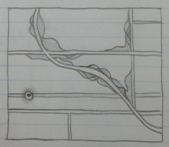
\includegraphics[scale=1]{figures/wire-1.png}
    \caption{Initial wireframe for histogram approach.}
    \label{fig:wire-1}
  \end{centering}
\end{figure}

\begin{figure}[htbp!]
  \begin{centering}
    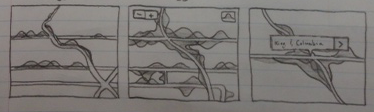
\includegraphics[scale=1]{figures/wire-2.png}
    \caption{Application wireframes showing interaction controls and pop-up menu.}
    \label{fig:wire-2}
  \end{centering}
\end{figure}

As can be seen in Figures \ref{fig:wire-1} - \ref{fig:wire-4}, various overlay techniques using both histograms and circular polygons on a map of a city were explored here in this early stage.
The histogram approach sought to model each vehicle (or small group of vehicles) on the road as a probability density function that could be moved along a road based on knowledge of traffic presence at each intersection, and speed limit data on each road.
More vehicles means more histograms, shown as translucent graphs which when overlaid, become more and more opaque, thus indicating a higher traffic density in that area.

\begin{figure}[htbp!]
  \begin{centering}
    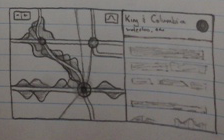
\includegraphics[scale=1]{figures/wire-4.png}
    \caption{Sketch of potential side menu for the Relay Interface application.}
    \label{fig:wire-3}
  \end{centering}
\end{figure}

Response for this concept was generally critical, as probability functions overlaid on a map were found to not be particularly easy to understand, at least not immediately at a glance.
It was evident at this stage that a simpler - more intuitive - visualization was needed for this application to be useful for both consumers and traffic engineers.

\begin{figure}[htbp!]
  \begin{centering}
    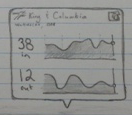
\includegraphics[scale=1]{figures/wire-5.png}
    \caption{Sketch of a detailed pop-up menu showing intersection data.}
    \label{fig:wire-4}
  \end{centering}
\end{figure}

Through exploration of the circular polygon heat-map concept, a more agreeable solution was found.
This concept modelled traffic data on a per intersection basis.
In other words, when an intersection is experiencing a high volume of traffic, a translucent circular polygon is triggered and overlaid onto a map of the city at the longitude and latitude of the intersection.
The size of the circle is positively correlated to the volume of traffic at the intersection.
A second degree of data is then shown through use of colour, to illustrate the performance of the intersection itself.
This gives insight into how well the intersection is moving traffic given it's high-volume state.
It was agreed upon that a well-performing high-volume intersection should receive a colour that is neutral, while a high-volume intersection with poor performance should emit a colour that indicates that something is wrong, such as orange or red.

It can also be seen in the figures that other components of the prototype application were accounted for in the wireframes.
These include interactions such as pop-up dialogues, highlighting routes and communicating intersections, as well as a side-panel for showing detailed metrics on intersection and overall city-wide traffic performance.
From this stage, the prototype moved to a mid-fidelity phase to further build out the concepts and refine the aesthetic of the application.

While not all of these early-stage concepts were used in the final product, the process of generating, critiquing, and refining multiple ideas proved valuable throughout the year.
These initial visualization concepts helped to spawn and guide future implementations, and helped attain a clear understanding of the data being presented.
The next step in the design process moved into a medium-fidelity stage, such that navigation and interaction could be explored at a deeper level.

\subsubsection{Medium-Fidelity Prototyping}
Through the use of prototyping software Balsamiq, a set of interactive mockups were created to both reflect the requirements of the application, as well as ideas and lessons learned from the previous wireframing stage.
In this prototype, the main tenets for the final version of the application were created in an illustrative form, to identify key architectural components and the user's interaction within.
By doing this in a medium that does not put too much focus on the specifics of visual design, it was easier to concentrate on the core features of the application, and how they satisfy (or dissatisfy) the original requirements. 

At this stage, the concept of data layers was explored.
Given that there are many varying metrics identified as important to target users (Traffic Engineers), and that these metrics all have a spatial or location-based relevance, the idea of turning on and off layers of data visualization overlaid on a map was critical in effectively demonstrating traffic data.
Metrics such as intersection Status, and Flow through an intersection were conceptualized at this stage, with some preliminary UI put together for interacting with these layers.
A screenshot of the mockup showing a Status visualization in the Relay app is presented in Figure \ref{fig:bals-1}. \\

\begin{figure}[htbp!]
  \begin{centering}
    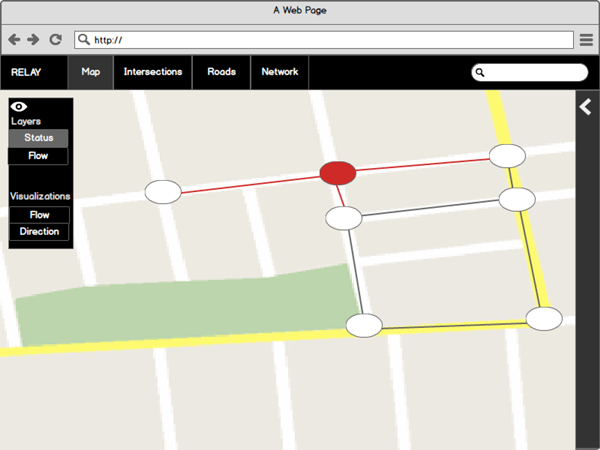
\includegraphics[scale=0.65]{figures/bals-1.png}
    \caption{Balsamiq mockup of a data layer in the Relay app.}
    \label{fig:bals-1}
  \end{centering}
\end{figure}

Additionally, as can be seen at the top of Figure \ref{fig:bals-1} the foundations for global app navigation were built out, in the form of a fixed header bar at the top of the screen.
This header serves many purposes, including branding for the app, search functionality, as well as tabbed buttons to move between contextually grouped pages.
Figure \ref{fig:bals-1} shows the active state of the Map button, while the main area of the screen contains a map with relevant data.

Further interaction design was carried out at this stage, in the form of a modular popup window, referred to as the Relay info box.
This info box was designed to present deeper metrics for an intersection, and appears when an intersection on the map is clicked.
This allows users to quickly inspect any intersection of interest and monitor time-series data in the context of a specific location.
Data provided at this stage includes a graph of the flow of traffic through the intersection in each of the cardinal directions, as well as a matching chart that provides predictive data into the near future, based on stochastic methods from the controller.
The status of the lights is shown, in addition to numerical car counts and the name of the intersection that has been clicked.
A Balsamiq mockup of the info box is presented in Figure \ref{fig:bals-2}. \\

\begin{figure}[htbp!]
  \begin{centering}
    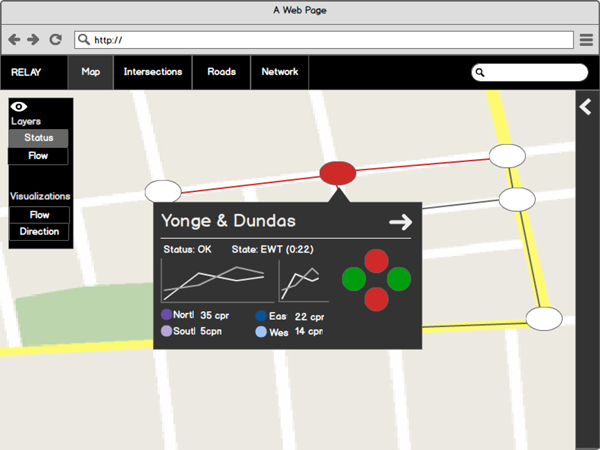
\includegraphics[scale=0.6]{figures/bals-2.png}
    \caption{Balsamiq mockup of the Relay info box.}
    \label{fig:bals-2}
  \end{centering}
\end{figure}

\begin{figure}[htbp!]
  \begin{centering}
    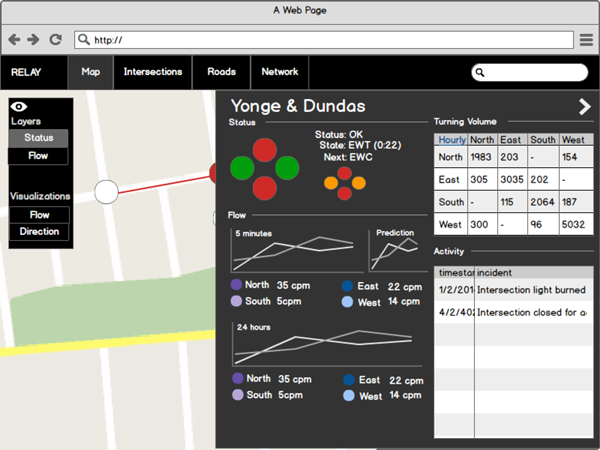
\includegraphics[scale=0.6]{figures/bals-3.png}
    \caption{Balsamiq mockup of the Relay dashboard.}
    \label{fig:bals-3}
  \end{centering}
\end{figure}

While the info box fulfills the need to browse intersections and provide quick snapshots of relevant intersection data, it was important for more advanced users to get an in depth look at this data, such that meaningful trends can be detected and acted upon.
It was necessary for these users - Traffic Engineers - to view metrics on intersection Location, Name, Type, State, In Flow, Out Flow, Predictions, and more.
To accommodate this large quantity of data, a dashboard was prototyped at this stage, setting a preliminary layout for each of the required metrics.
This dashboard slides across the screen from the right by pressing the arrow in the info box, and can then be toggled back and forth with the controls in the upper right corner of the screen.
A Balsamiq mockup of the dashboard can be found above in Figure \ref{fig:bals-3}.
As various intersections are selected on the map, the dashboard updates it's information to reflect that of the intended location.
Time-series graphs update in real-time as data feeds through the system, and an activity log hosts the history of noteworthy incidents at the selected intersection.

With these views on the Map screen prototyped in medium-fidelity, the design progressed into other areas of the application.
Moving through the global navigation buttons along the header, an Intersections page was mocked up.
The goal of this page is to give Traffic Engineers a holistic view on their network, as well as the ability to filter/search and target individual intersections.
This text-based search also allows for insight into any particular intersection by name, as well as the ability to find important groups of intersections or main arteries with many cross streets.
This is important because it allows users to locate intersections in two ways: spatially on the map, and now textually in the intersections table.
A mockup of the Intersections page is shown in Figure \ref{fig:bals-4}, with placeholder data in the intersections table. \\

\begin{figure}[htbp!]
  \begin{centering}
    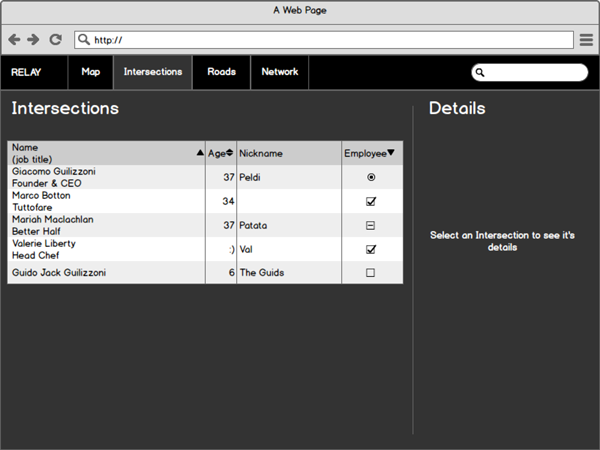
\includegraphics[scale=0.65]{figures/bals-4.png}
    \caption{Balsamiq mockup of the Intersections page.}
    \label{fig:bals-4}
  \end{centering}
\end{figure}

Finally, the medium-fidelity prototyping stage moved on to build out a layout and basic information for a Network page.
The intention of this page is to provide details similar to what would be shown in the info box or dashboard of an intersection, but for the entire network as a whole.
This allows Traffic Engineers to view, understand, diagnose, and make decisions for the network on a macro level, in addition to the finer look provided on a per intersection basis.
A mockup of the Network page is shown in Figure \ref{fig:bals-5}. \\

\begin{figure}[htbp!]
  \begin{centering}
    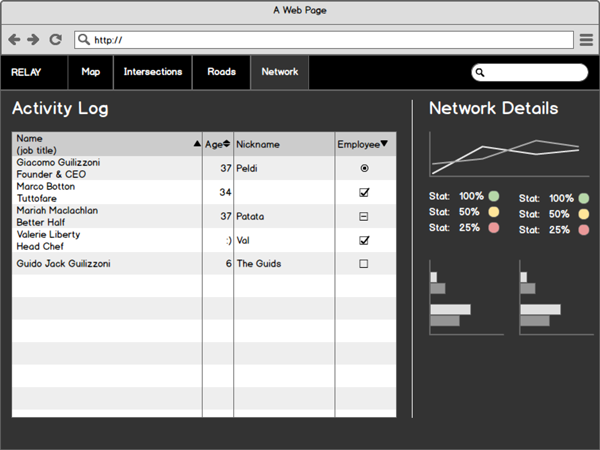
\includegraphics[scale=0.6]{figures/bals-5.png}
    \caption{Balsamiq mockup of the Network page.}
    \label{fig:bals-5}
  \end{centering}
\end{figure}

As can be seen in Figure \ref{fig:bals-5}, a large activity table is provided on the Network page, to highlight issues that occur at all intersections in the network.
These issues include accidents, power outages, abnormal volumes, and more.
Additional detail can be seen on the right hand side of the screen, with quantitative network data placed in charts and numerical tables, and colour-coding of network statuses explored at this stage.

Overall, the medium-fidelity prototyping stage was essential in moving the design of the Relay application forward towards its final state.
With functional requirements set in place, and now a strong roadmap of UI elements, navigation, page layout, and interactions to fulfill the requirements, the application was ready to be built in a high-fidelity form, as described in the following section.

\subsubsection{High-Fidelity Prototyping}
In preparation for the development of the Relay application, the design of the environment moved into a final high-fidelity prototyping phase.
This stage involved a major visual overhaul of the application, focusing on the definition of a unique design language to bring Relay together as a cohesive product.
Considerations at this stage include the creation of a custom grid structure, typography, colour, branding, the development of data visualization layers, and repurposing the search functionality in the app.
The high-fidelity design was done in Adobe Photoshop, Illustrator, and in the browser using HTML/CSS and JavaScript.
These tools allowed for highly accurate creation of assets, development of colour scheme, precise layout of visual elements, and more.

The branding for Relay was created in two main components: the logo, and the typesetting.
The logo is a custom glyph used in the application to denote the state of the signal at an intersection.
It contains four dots in a diamond pattern, with two fully-coloured dots positioned vertically, and two empty dots with a medium-weight stroke positioned horizontally.
In the application, this glyph would represent the flow of traffic in an East-West manner, while North-South traffic is halted at a red light.
This was selected to represent Relay as it both subtly represents what the application does, and provides important information to users in a modern and clean way.
The final Relay branding is shown in Figure \ref{fig:relay-logo}. \\ \\

\begin{figure}[htbp!]
  \begin{centering}
    
\includegraphics[scale=0.7]{figures/relay-logo.png}
    \caption{High-fidelity rendering of the Relay branding.}
    \label{fig:relay-logo}
  \end{centering}
\end{figure}

The typesetting was done to represent Relay in a way that would be clear, trustworthy, confident, readable, and modern.
The use of custom letter positioning through tracking and kerning methods aided this, while promoting clarity and confidence with the capitalization of each letter in the word.
Open Sans, a typeface that is freely available to the public, was utilized for the clean and readable aesthetic it provides.
As a sans-serif font set at a semi-bold weight, each letter is clear from any distance, at many sizes, on both screen and in print.
This also gives the branding a modern feel, as many serifed fonts are often associated with older, more classical and formal scenarios.

The high-fidelity design of the application itself began at a structural level, to set the basis for a consistent, coherent, and unique interface.
A grid structure was optimized for a 1440 x 900 pixel resolution screen - a common resolution on modern screens, and the dimensions of the screens used for the Symposium demo.
The grid was based upon units of 16 pixels, which was decided to be the lowest common denominator for icon and type sizing to ensure usability from many angles and distances.
With a grid structure in place, all following design decisions then had a reference point to follow from.
This aided in the purposeful use of negative spacing, symmetry, and balance of each screen composition.
The grid on a blank canvas is shown in Figure \ref{fig:dot-grid}. \\

\begin{figure}[htbp!]
  \begin{centering}
    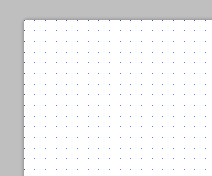
\includegraphics[scale=1]{figures/dot-grid.png}
    \caption{16 pixel grid foundation for the Relay user interface.}
    \label{fig:dot-grid}
  \end{centering}
\end{figure}

The first consideration in developing the design language for the application was the typography.
Just like the branding, the typography was intended to be clear and readable, but also neutral in tone.
Neutrality of the type allows for clear representation of the content itself, which is highly important in such a data-heavy application.
As a critical element of the user interface, particular attention was paid to hierarchy of type sizes and weights, all deriving from a smallest line-height of 16 pixels, used in small data labels and body.
The typeface Helvetica Neue was used, as it is well-known to provide very clear and readable text at many sizes, with a neutral tone.
Additionally, it is a common typeface used in the signage of many major cities around the world.
This gives the application a recognizable and associative feeling, which is especially important for an application that deals with traffic conditions in urban areas.
An example of an intersection name set in 24pt Helvetica Neue Bold is shown in Figure \ref{fig:name}. \\

\begin{figure}[htbp!]
  \begin{centering}
    
\includegraphics[scale=1]{figures/name.png}
    \caption{An intersection name set in 24pt Helvetica Neue Bold.}
    \label{fig:name}
  \end{centering}
\end{figure}

The high-fidelity prototyping process continued with the development of colour-scheme for the application.
Given the importance of visualizing data in the Relay app, it was decided that all non-data elements of the UI - the map, modular overlays, and header, for example - should be subdued and clearly grouped together as functionally similar elements.
To accomplish this, a black and white UI was established for all control elements, providing a clean environment for navigation, while vibrant, highly-saturated colours were used for charts and data layers.
This technique effectively created a high-contrast environment where areas that require visual focus, attention, and thought - i.e. the data - were the most salient elements on the screen, and any layout or navigational components were done in a clear black and white manner, similar to signage found on the streets of many major cities.
Therefore, all contextually similar elements were easily grouped and identifiable through their similarities or differences in colour.
An example of a chart showing the flow of traffic through an intersection over time is illustrated in Figure \ref{fig:chart}.
Notice the vibrancy of the coloured data, and its contrast with the structural page elements surrounding it. \\

\begin{figure}[htbp!]
  \begin{centering}
    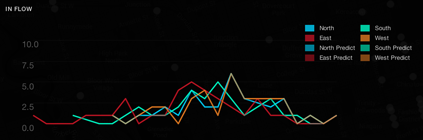
\includegraphics[scale=0.9]{figures/chart.png}
    \caption{A chart showing the flow of traffic through an intersection over time.}
    \label{fig:chart}
  \end{centering}
\end{figure}

The data visualization layers were next to be developed at the high-fidelity stage.
These visualizations took the form of heat maps, as well as quantitative, relative, and boolean glyphs, representing data on the Status, Flow, and Queue Length at a given intersection.
The first visualization layer, showing the Status of intersections, used small dot glyphs of different colour to display the boolean status of a light.
By overlaying a dot at each intersection, with a corresponding white or red colour to denote proper working condition vs. an error, such as a power outage, an easily digestible visualization was created.
This empowers Traffic Engineers to easily monitor their network, and to detect any anomalies that may have occurred.
A screenshot of the Status layer is shown in Figure \ref{fig:status}. \\

\begin{figure}[htbp!]
  \begin{centering}
    
\includegraphics[scale=0.9]{figures/status.png}
    \caption{A screenshot of the intersection Status data layer.}
    \label{fig:status}
  \end{centering}
\end{figure}

The second data layer to be designed was a heat map representing the flow of traffic through intersections.
This was accomplished on a per-intersection basis, and was intended to provide a macro view of the relative traffic density across areas of the city.
This view is most useful for those looking for an overview of general traffic conditions, such as a browsing Traffic Engineer, or a consumer looking to plan a route through the city.
A screenshot of the first Flow visualization layer is shown in Figure \ref{fig:flow-1}.

\begin{figure}[htbp!]
  \begin{centering}
    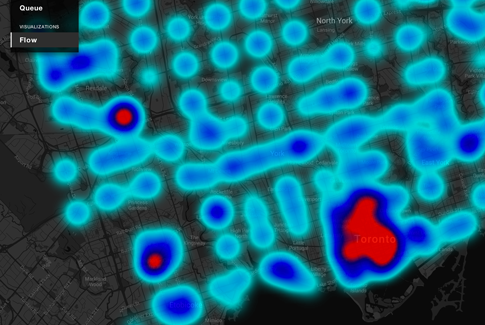
\includegraphics[scale=0.9]{figures/flow-1.png}
    \caption{A screenshot of the flow per-intersection heat map.}
    \label{fig:flow-1}
  \end{centering}
\end{figure}

Following this Flow visualization, a second implementation of traffic flow was developed, this time looking at flow between intersections, rather than at or through any particular intersection.
This was accomplished by taking predictive data from the controller, and approximating the position of cars along roadways given the knowledge of their entry and exit directions from each intersection.
Each car is plotted as a low-opacity glyph of concentric circles, with a bright green core, a lighter green exterior, and a soft blue outline, denoting the estimated nature of the position of any given car.
Given the large number of vehicles to be accounted for, a low opacity was selected for each individual glyph, so that as they overlap with one another, the intensity of the colour increases so as to illustrate the increasing density of traffic in an area.
A screenshot of the Flow between intersections data layer is shown in Figure \ref{fig:flow-2}.

\begin{figure}[htbp!]
  \begin{centering}
    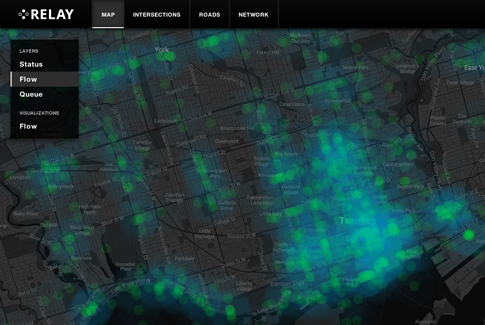
\includegraphics[scale=0.9]{figures/flow-2.png}
    \caption{A screenshot of the flow between intersections heat map.}
    \label{fig:flow-2}
  \end{centering}
\end{figure}

As can be seen in Figure \ref{fig:flow-2}, the natural visualization of major roadways and arteries through the cities is evident, which is an important result of this visualization.
A wide range of traffic patterns can be derived from this, thanks to the high-resolution of data points that give a continuous feel to the data, as opposed to the limited two-stage discrete options currently available through applications such as Google and Apple Maps.

Finally, the final visualization layer looked to showcase the data representing Queue Length or average wait time at an intersection.
The goal of this visualization was to produce glyphs that could show both quantitative measures, as well as give a sense of relative weighting between intersections.
A four-pronged glyph was developed, with three short prongs extending in the East, South, and West directions, while a variably sized prong extends to the North.
The length of the North prong corresponds to the average wait time at a given intersection, while the three shorter prongs are of equal length and serve as a stand for the quantitative North measure.
This creates a pseudo 3-dimensional effect, and gives the user a unique look at the changing landscape of queue lengths in the city - similar to how a city skyline may look with many tall buildings.
A screenshot of the Queue Length visualization layer is shown in Figure \ref{fig:queue}.

\begin{figure}[htbp!]
  \begin{centering}
    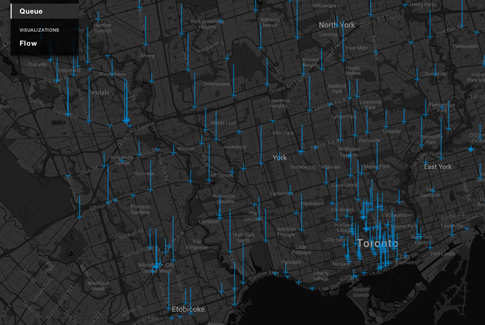
\includegraphics[scale=0.9]{figures/queue.png}
    \caption{A screenshot of the average queue length at each intersection.}
    \label{fig:queue}
  \end{centering}
\end{figure}

Following the design of the data visualization layers, the high-fidelity stage looked at the search functionality of the application, and focused attention on repurposing its form to better reflect its function.
Previous prototypes held the search bar in the header across all pages of the application.
This proved to be troublesome, as some pages did not require any search functionality, while the ones that did actually served as text-based filters within the context of the current page.
The high-fidelity design saw the removal of the search bar from the global navigation header, and into the upper section of the Intersections and Network pages.
This way, the text-based tables found on these pages could be easily searched/filtered, without the confusion of entering text into the global header, where a new page would be the expected result.

An additional feature that made its way through the high-fidelity phase is the Connection Status window.
This window is activated through the gear icon in the top right corner of the screen, and is useful for monitoring the status of the connection between the front-end and back-end of the application.
This window is positioned in the top-right of the screen so as to avoid covering any important visual elements, and is padded in from the top and right sides of the screen to maintain access to the dashboard toggle button.
The connection status window identifies where the data is coming from: either through a Web Socket or through the application's REST API.
It also identifies time since the last data update, both locally on a selected intersection, and globally over the entire network.
A screenshot of the Connection Status window is shown in Figure \ref{fig:connection}.

\begin{figure}[htbp!]
  \begin{centering}
    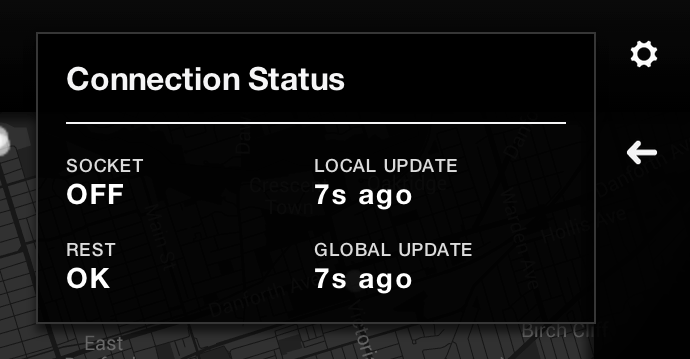
\includegraphics[scale=0.6]{figures/connection.png}
    \caption{A screenshot of the connection status window.}
    \label{fig:connection}
  \end{centering}
\end{figure}

Lastly, the intersection dashboard was refined at a high-fidelity stage.
The specific metrics contained in the dashboard were iterated on and refined from the medium-fidelity stage to accurately reflect the data coming from the back-end controller.
This involved splitting the Flow metric into In-Flow and Out-Flow at an intersection, showing the current and next intended State of the traffic lights, and providing a new Turn Predictions matrix, which gives the predicted quantity of cars moving through each permutation of turns based on stochastic data from the back-end.
In-line with the medium-fidelity prototype, the Activity Log is provided giving consideration to readability and interaction, with subtle hover states on individual table rows to improve salience of desired fields.
Additional information includes the Intersection ID and the Intersection Type, two identifiers that are often important to Traffic Engineers.
A screenshot of the high-fidelity dashboard is shown in Figure \ref{fig:dashboardt}. \\

\begin{figure}[htbp!]
  \begin{centering}
    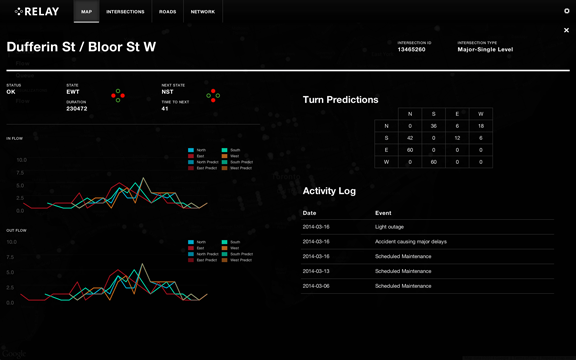
\includegraphics[scale=0.73]{figures/dashboard.png}
    \caption{A screenshot of the Relay intersection dashboard.}
    \label{fig:dashboardt}
  \end{centering}
\end{figure}

With these elements in place, the final developmental/functional touches to the Relay application were ready to be built for the demo, as showcased on Symposium day.
As a unit, the application is held together using the modular design elements described above, which makes the application easily scalable and modifiable for individual implementations or changing metrics and requirements.
With a unique and well-defined design language established, further extrapolations of this implementation have a library of best practices and UI elements that can be carried forward into new scenarios.

\subsection{Application Architecture}

Application interfaces for critical infrastructure must be highly robust and reliable. Furthermore, it is important the the systems are able to scale in order to accomodate the inevitable growth of the system. These main ideas drove the design of the front-end (web application) application architecture. 

Given the breadth of choices in software technology, it was necessary to use a quantifiable selection process for determining the appropriate solutions from a group of candidates. The three main areas of the front-end application which required such a process are the Framework, Mapping Library, and Visualization Library. The selection process for these is discussed in the following sections.

\subsubsection{Framework Selection}

Software frameworks are code libraries which provide functionality that enables developers to more easily implement a specific software pattern. One of the most common software patterns is the Model-View-Controller (MVC) pattern, which is commonly used in complex and large software applications to ensure the application is reliable, structured, and can scale effectively. Similarly, front-end software frameworks allows for the development of structered and scalable applications by providing software pattern untilities. Given the critical nature of our application, it was determined that the use of a framework would be appropriate for ensuring the scalability and reliabilty of the application.

Four JavaScript frameworks were selected for comparison. Javascript MVC is a mature, well-known front-end MVC implementation which is build off of jQuery, a JavaScript Utility Library, which offers a well-rounded feature base. DOJO is another mature and well-known framework which does not offer an MVC-style framework, yet is class-oriented. Backbone.JS is a relatively new Model-View (MV) framework built off of the Underscore.js utility library. Finally, Angular.js is a new and highly functional front-end framework which loosely follows an MVC pattern.

The frameworks are scored across five weighted features. The scores are justified and a winning framework is selected.

\begin{enumerate}

\item \textbf{Size} - The use of large JavaScript libraries can cause performance issues within the application. The selected library should be as small as possible. Candidate frameworks will be assesed based on the size of their encompassing code files. This feature has been given a weight of 0.5.

\item \textbf{Independance} - The selected framework should be self-contained and not require many prerequisite JavaScript Libraries in order to function. The presence of many prerequisite libraries increases the size of the application and will slow down performance. Candidate frameworks are assesed based on the number of prerequisite frameworks and plug-ins required for the framework's application within the proposed solution. This feature has been given a weight of 0.5.

\item \textbf{Functionality} - The selected JavaScript framework should provide a rich set functionality which is not available within the native Javascript language. Important functionality includes utility functions, templating, Document Object Model (DOM) binding, client-server communication methods, and data structure classes. Candidate frameworks are assessed based on the both the quantity and quality of the functionality provided, in the context of the proposed soluction. This feature has been given a weight of 0.8, as it is important that the framework provide sufficient functionality to implement the solution.

\item \textbf{Modularity} - It is important that the selected JavaScvript framework supports the creation of modular code, given the complexity of the proposed solution. The selected MVC framework should encourage an exablished code pattern, such as and MV- or MVC-style structure. Candidate frameworks are assesed based on their similarity to known software architecture patterns, such as MV or MVC. Due to the importance of scalability and modularity in the proposed solution, this feature has been given a weighting of 0.8.

\item \textbf{Implementation Overhead} - The selected JavaScript framework should not require excessive amounts of overhead code in order to successfully suit the needs of the proposed solution. The selected framework should have as little overhead as possible. Candidate frameworks are assessed by examining tutorial code implementations for each framework, to determine the proportion of development required as overhead compared to application-specific code. This feature has been given a weight of 0.5.

\end{enumerate}

The frameworks are presented in a weighted decision matrix below. Each attribute is weighted out of 5 points for each of the candidate frameworks. Weightings for each attribute are on a scale from 0 to 1.

\begin{table}
\centering
    \begin{tabular}{l|llll}
    ~                             & Angular.js & \textbf{Backbone.js} & DOJO    & JavaScript MVC \\ \hline
    Size (0.5)                    & 5 (2.5)    & \textbf{3 (1.5)}     & 2 (1)   & 2 (1)        \\
    Independence (0.5)            & 5 (2.5)    & \textbf{4 (2)}       & 3 (1.5)   & 4 (2)          \\
    Functionality (0.8)           & 3 (2.4)    & \textbf{5 (4)}       & 4 (3.6)   & 4 (3.6)          \\
    Modularity (0.8)              & 2 (1.6)    & \textbf{4 (3.6)}     & 4 (3.6) & 4 (3.6)        \\
    Implementation Overhead (0.7) & 4 (2.8)    & \textbf{4 (2.8)}     & 3 (2.1) & 4 (2.8)        \\ \hline
    Totals                        & 11.8       & \textbf{13.9}        & 11.8    & 13.0           \\
    \end{tabular}
\caption{Weighted Decision Matrix for JavaScript Framework Selection}
\label{table:framework-matrix}
\end{table}

Angular.js is the smallest candidate framework at 36kb. Angular.js also has no dependancy JavaScript libraries, and is thus completely independant. Although Angular.js offers rich DOM and interaction functionality, it provides few utility features for data structures and architectures. Angular.js does not follow a rigid MVC or MV structure, which was a major downfall for the framework. Anjular.js does not require much overhead code to implement, primarily because it does not follow a rigid software architecture, and thus is more functionally-oriented.

The Backbone JavaScript framework is 64kb in size. Backbone.js relies on Underscore.js and jQuery.js two relatively large JavaScript utility libraries. However, both of these libraries will be used in the application regardless of the choice of framework, thus are not direct detriment of this candidate. Backbone.js follows a MV framework style, where both controller and view functionality are both kept in the view. This pattern is a good comprimise between no framework and an extremely heavy MVC structure. Backbone.js's two utility libraries provide rich functionality for working with the DOM model, and structured objects. Furthermore, Backbone provides a native collection-oriented pattern developed specifically for handling large numbers of similar objects, which fits well with the applications need to support many intersection and road models. Finally, Backbone.js has minimal development overhead considering it's MV structure, as Backbone.js provides a range of default functionality for it's classes.

The DOJO JavaScript framework is 155kb in size, making it the largest of the candidate frameworks. DOJO requires no prerequisite JavaScript Libraries, yet many of DOJO's features are in add-on libraries. This reduces the effectiveness of DOJO's core code, yet means a wider range of features are available as the feature set distributed and open. However, DOJO's functionality is not aimed specifically at dealing with large collections of data, and does not offer strong support for client-server synchronicity. In terms of modularity, the DOJO framework supports the creation of class objects yet does not explicitly support an MV- or MVC-style framework. DOJO requires a significant amount of implementation overhead, which makes it suitable for extremely large and diverse applications. However, this level of overhead is less suited to the complex yet relatively consistent nature of our application with respect to object and data needs.

JavaScript MVC is 105kb in size. JavaScrvipt MVC relies on the jQuery.js JavaScript library, however this library is already a requirement for the proposed solution. JavaScript MVC is composed of four sub-frameworks, each of which specializes in a different set of features, and together provide sufficient functionality for the proposed solution. However, like DOJO, JavaScript MVC lacks the specific functionality for dealing with large amounts of similar objects. As suggested by the name, JavaScript MVC follows a strong MVC model in it's implementation.

As seen in table \ref{table:framework-matrix}, Backbone.js is the winning candidate. Backbone is not the smallest candidate, yet it's feature set and MV framework fit well with the needs of the proposed solution. Specifically, Backbone's use of already-implemented JavaScript utility libraries to provide enhanced data structure tools and algorithms, as well as it's specialized collection template for dealing with large amounts of data objects. Furthermore, Backbone.js provides functionality for client-server communication for said collection structures. Finally, the overhead associated with Backbone.js is acceptable given the strong fit of the functionality with that of the proposed solution.

\subsubsection{Mapping Library Selection}

Next, a front-end mapping library needed to be selected. The proposed solution required that information be viewed in a geographic context. Thus, it was necessary to select a client-side library which would support these needs. Generally, it was important the the library be highly-customizable, as the data presentation layers would be completely customized. Furthermore, the library had to be high-performance to support the needs of our application. Finally, it was necesary to find a map hosting service which could support the library, as setting up a hosting service was not in the scope of this solution.

\begin{enumerate}

\item \textbf{Style Customizability} - The selected mapping candidate should be highly customizable. Colour and styling for map features such as roads, buildings, water, and land must be allowed. This feature has been given a weight of 0.5, as it is not crucial yet still important to the aesthetic value of the interface.

\item \textbf{Feature Customizability} - The selected mapping candidate must allow for the customization of built-in features, such as markers and info boxes. Markers should be completely customizable, through the use of either a scalable vector graphic (SVG) or HTML and CSS. Info boxes should be customizable using HTML, CSS, and JavaScript. This feature has been given a weight of 0.7 for it's importance in defining the customizability of crucial interface features.

\item \textbf{Layer Customizability} - The selected mapping candidate must allow for the customization of map data layers. The candidate must support multiple simultaneous layers of data. It should also support the display of both point-based and vector-based data. This feature has been given a weight of 0.9, as the value of the application is directly related to the presentation of the various data layers.

\item \textbf{Tile Hosting Support} - The selected mapping candidate must either support tile hosting as part of its service, or be compatible with an existing tile hosting service. Ideally, the selected candidate offers both tile hosting and serving in the same package for convenience. This feature has been given a weight of 0.6, as it is not a crucial feature yet saves significant effort if present.

\item \textbf{Price} - The selected mapping candidate must be cost effective. The service should be free, or minimize the cost of tile serving and hosting. This feature has been given a weight of 1 due to the highly restrictive budget for the proposed solution.

\end{enumerate}

Four Mapping Libraries were considered as potential candidates: Google Maps API, Leaflet.js, MapBox, and TileMill in conjunction with CloudMade.

The Google Maps API is the industry standard of mapping libraries. It is the same framework which runs Google Maps, and is thus well-supported and reliable. The Google Map API allows for styling customizations on-the-go throught it's JavaScript API. Unfortunately, not all aspects of the map are stylable. The API provides functionality for both markers and info boxes. The Google Maps API allows for custom CSV marker icons, however the info box is not easily customizable. However, Google Maps does offer a plug-in info box, which is fully customizable. Tiles are hosted directly through Google Maps, requiring no extra work for tile hosting support. Finally, the Google Maps API is a free service with very high courtesy limits.

Leaftlet.js is a map-oriented JavaScript Library which provides a variety of map-related features on top of a tile service. Leaflet.js does not host map tiles, and thus it must be used in conjunction with a tile hosting service such as CloudMade. As such, styling the map must be done through a CloudMade's third party service which is restrictive in styling. Leatlet.js offers rich map functionality, including markers and info boxes. Furthermore, leaflet.js' map features are highly-customizable, as it is an open-source project. However, Leaflet.js id not geared towards handling data layers. Leaflet.js is a free library.

Mapbox is a new JavaScript mapping library which works in conjunction with TileMill, a tile styling styling service. TileMill is designed specifically for creating highly-customized map styles, and thus offers very rich styling capability. Due to MapBox's immaturity as a platform, it's feature set is limited and not very customizable. The MapBox JavaScript Library is not structured towards handling data layers, rather individual data points. Furthermore, TileMill tiles must be hosted using a third part platform, or through MapBox directly, which required a paid membership for the service.

\begin{table}
\centering
    \begin{tabular}{l |r r r l}
    ~                             & \textbf{Google Maps API} & Leaflet.js \& CloudMade & MapBox \& TileMill \\ \hline
    Style Customizability  (0.5)  & \textbf{3 (1.5)}         & 3 (1.5)                 & 5 (2.5)            \\
    Feature Customizability (0.7) & \textbf{4 (2.8)}         & 5 (3.5)                 & 3 (2.1)            \\
    Layer Customizability (0.9)   & \textbf{5 (4.5)}         & 4 (3.6)                 & 3 (2.7)            \\
    Tile Hosting Support (0.6)    & \textbf{5 (3.0)}           & 3 (1.8)                 & 3 (1.8)            \\
    Price (1)                     & \textbf{5 (5.0)}           & 4 (4.0)                   & 3 (3.0)              \\ \hline
    Total                         & \textbf{16.8}            & 14.4                    & 12.1               \\
    \end{tabular}
\caption{Weighted Decision Matrix for Mapping Library Selection}
\label{table:mapping-matrix}
\end{table}

The candidate mapping libraries are compared in Table \ref{table:mapping-matrix}. The Google Maps API is the winning mapping library. Although the Google Maps Library lacks full native customizability for both it's map styling and map features, sufficient customizability is found within the native functionality and through the use of add-on libraries. The Google Maps API provides excellent data layer functionality, which is unparalled in feature breadth and support. Finally, the Google Maps combined tile hosting and JavaScript functionality provided within a free service make it the clear choice.

\subsubsection{Visualization Library Selection}

Given the proposed solution's heavy focus on data presentation and visualization, it was important to select a visualization library which supported a wie range of data visualization formats. It was necessary to select a library which allowed for heavy style customization, including line format, colours, grid styles, and legend displays. Considering that traffic information exists in the temporal space, it was imporant that the library handle time series data well. Specifically, functionality for handling timestamp formatting and real-time or high-frequency updating.

The candidate visualization libraries are assessed across 5 feature categories.

\begin{enumerate}

\item \textbf{Prerequisites and Add-Ons} - The selected visualization library should require minimal additional plug-ins or libraries to run. All of the necessary functionality should be available within the core library files. Candidate libraries will be assessed based on the number of additional files or libraries required to perform. This feature has been given a weight of 0.5, as the functionality of the library is relatively more important than the quantity and size of the library's dependancies.

\item \textbf{Implementation Complexity} - The selected visualization should minimize the amount of code required to produce the necessary visualization. Unnecessarily long setup scripts may cause performance issues in the code. Candidate mapping libraries will be assesed by examining example code and tutorials in order to understand the complexity of visualization implementation.This feature has been given a weight of 0.8, due to the frequency and extent of visualization use within the proposed solution.

\item \textbf{Time-Series Support} - The selected visualization library should have rich time-series support. The library should support timestamps in various data formats and allow for the display of time values in a variety of formats. Candidate mapping libraries will be assessed based on the extent of the documented time-series formatting functionality available for the library. This feature has been given a weight of 0.9, as time-series support is crucial for the proper display of information within the proposed solution.

\item \textbf{Style Customizability} - The selected visualization library must allow for highly customized visualizations. The library should allow for the customization of visualization style, line style, legend style and placement, grid style and placement, and axis style and placement. Candidate mapping libraries will be assessed based on the extent of documented customizable features available for the library. This feature has been given a weight of 0.8, due to the importance of data presentation style in the success of the proposed solution.

\item \textbf{Ease of Updating} - The selected visualization library must support real-time updating of the data within the visualization. The library should either explicitly support data updating through JavaScript methods, or allow for the replacement of the data object and the redrawing of the visualization. Candidate libraries will be assesed based on the perceived presence of such functionality within the library documentation. This feature has been given a weight of 0.9, as the proposed solution relies on the real-time display of information.

\end{enumerate}

Four JavaScript-based visualization libraries were assessed as candidates.

Chart.js is an HTML5-based visualization library, focused on delivering implementations of several core data presentation formats, e.g. bar charts and line charts. Chart.js is a stand-alone library, requiring no outside code. The implementation of visualizations in Chart.js is easy and requires minimal amounts of code. Chart.js does not support any formatting for axis labels, including support for date formatting and time-series support. Chart.js provides an intermediate amount of formatting options for visualizations, however the restriction of the library to 6 main visualization formats limits the presentations options while using this library. Furthermore, Chart.js does not support the updating of chart data in any way, and would require the chart to be recreated in order to display new data.

D3, or Data-Driven Documents, is the most well-known and feautre-rich HTML visualization library today. D3 provides an extremely wide range of visualization formats which are completely customizable. D3 has no pre-requisite libraries, and is a stand-alone library. D3's main downfall is the complexity of implementaion, as basic data presentations can require up to 300 lines of code. As an extension of D3's extreme customizability, it is possible to use time-series data, however the library provides little native formatting support. D3 provides the widest range of visualization options by far. Finally, D3's support of data updating depends on the visualization method used, however it is generally poor due to the static nature of the library.

Flot is a JavaScipt-based visualization library built on top of the jQuery utility library. Flot is a medium-complexity visualization library which emphasizes informative and real-time visualizations. As mentioned, the Flot library requires jQuery to run, however jQuery is already a prerequisite for multiple other libraries and feature in the proposed solution. Flot charts are not designed to be extremely easy to implement; their implementation complexity is significant, yet more efficient than other candidates and understandable given the functionality available. Flot natively offers moderate time-series formatting support: Flot accepts JavaScript timestamps as time-series data, and is able to format said data in a variety of styles. With the addition of a jQuery plugin, the range of styles is greatly increased. Flot provides a moderate amount of customizability for their data presentations. However, due to the open-source nature of Flot, the inner styling variables are publicly known, which allows them to be customized far beyond what is suppored through public JavaScript methods. Finally, Flot handles data updating very well, with explicit JavaScript functions for updating data objects and re-rendering visualizations.

Rickshaw is a new, static visualization library build using D3 functionality. It aims to offer less complex implementations of basic data visualizations using the D3 framework. Obviously, D3 must be loaded in order for Rickshaw to run, which brings the negative performance implications of loading such a large library as D3. Rickshaw data presentations are exceptionally easy to define and require minimal code. However, the immaturity of the library means that only a few plotting styles are supported, greatly limiting the library's capability. Furthermore, Rickshaw is a private library and is thus less accessible to customizing beyond the limited exposed styling options. Rickshaw does provide time-series formatting support, however it is limited in scope and buggy as the library is not yet a mature project. Finally, due to the static nature of the underlying D3 platform, the Rickshaw library has no support for updating the data object, and thus would require the recreation of the visualization.

\begin{table}
\centering
    \begin{tabular}{l | r r r r}
    ~                               & Chart.js & D3      & \textbf{Flot}    & Rickshaw \\ \hline
    Prerequisites \& Add-Ons (0.5)  & 5 (2.5)  & 5 (2.5) & \textbf{4 (2.0)} & 4 (2.0)  \\
    Implementation Complexity (0.8) & 4 (3.6)  & 1 (0.8) & \textbf{3 (2.4)} & 5 (4.0)  \\
    Time-Series Support (0.9)       & 1 (0.9)  & 3 (2.7) & \textbf{5 (4.5)} & 3 (2.7)  \\
    Style Customizability (0.8)     & 2 (1.6)  & 5 (4.0) & \textbf{4 (3.6)} & 3 (2.4)  \\
    Ease of Updating (0.9)          & 1 (0.9)  & 2 (1.4) & \textbf{4 (3.6)} & 1 (0.9)  \\ \hline
    Total                           & 9.5      & 11.4    & \textbf{16.1}    & 12.0     \\
    \end{tabular}
\caption{Weighted Decision Matrix for Visualization Library Selection}
\label{table:visualization-matrix}
\end{table}

Assessment of the candidate visualization libraries is done through a Weighted Decision Matrix, as seen in Table \ref{table:visualization-matrix}. As seen in Table \ref{table:visualization-matrix}, Flot is the winning visualization candidate. Flot's ecxceptional functionality with regards to time-series data and data updating fit well with the needs of the proposed solution. Furthermore, the Flot visualization library provided a suitable balance of complexity and customizability for the proposed solution.

\subsubsection{Architecture Development}

The architecture for the front-end application saw three major iterations. Each phase represents a more complex yet refined application architecture. Tables \ref{fig:iteration1}, \ref{fig:iteration2}, and \ref{fig:iteration3} document the Javascript architecture at each iteration. This section only discusses the progression of the JavaScript class architecture, and does not discuss the HTML or CSS development which happened in parallel. However, all other front-end development was done to support the JavaScript class structure, and thus discussion of their implementation is not necessary.

Due to the use of Backbone.js as the JavaScript framework, the application follows an MV architecture, where only models and views exists as distinct classes, and controller functionality is included in the view object. Backbone.js includes a specific model pattern called a collection, which is an object responsible for handling multiple models of the same class. The solution leverages the functionality provided by the collection pattern, and they have been appropriately categorized in the architecture diagrams. However, collections are similar to models in the sense that they have no controlling functionality, and thus are treated like models in the sense that each as an accompanying view class to handle it's controlling functionality.

The 'User Entry' mark within the class diagrams indicates the entry point to the initialization of the JavaScript code. This is done using a call to the script (iteration 1) or through the initialization of the indicated class object (iterations 2 and 3), which then progressively initializes all other classes within the structure. The arrow direction indicates the direction of ownership within the classes. That is, class A pointing to class B indicates that class A owned one or multiple instances of Class B. At the bottom of each diagram, database connection points are indicated. The presence of a line between a model and a database indicates the ability for the model to query the database. Finally, views which are directly owned by a collection view are stacked. This is to show the collection view's 1 to n relationship with the view classes in the implementation.

The first major implementation was a proof-of-concept interface developed for the Fall Demonstration and Presentation. The goal was a low-fidelity simulation of the core functionality in the solution. Thus, the code was developed in a less-structured manner so it could be changed quickly as various implementation strategies were tested. As seen in Figure \ref{fig:iteration1}, all functionality was developed in a single, classless script. No specific class pattern was implemented at this stage.

\begin{figure}[htbp!]
  \begin{centering}
    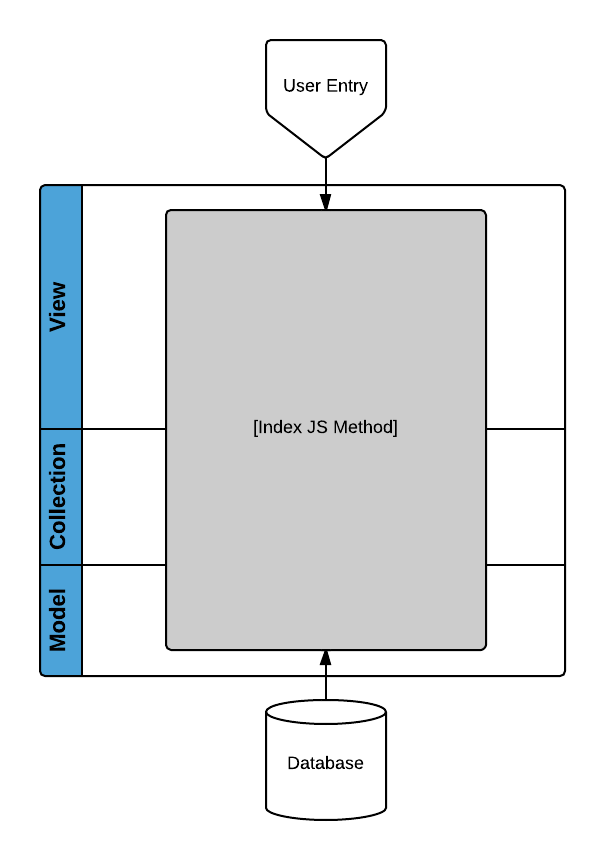
\includegraphics[scale=0.25]{figures/Iteration-1.png}
    \caption{An architectural diagram for Iteration 1.}
    \label{fig:iteration1}
  \end{centering}
\end{figure}

The second major implementation was completed for the Winter Demonstration and Presentation. A more mature class architecture had been developed, seen in Figure \ref{fig:iteration2} as many of the necessary utility libraries had been selected. Furthermore, Backbone.js had been selected as the JavaScript framework of choice, and significant effort had been made into transitioning the original functionality into the Backbone.js pattern.

The App View class is primarily responsible for handling the initialization of the application, and acts as a wrapper for all other functionality. This iteration contained a single screen, and the screen was approptiately given a View class to manage it's interface and interactions with the model. Furthermore, intersections pulled from the database were stored in a Collection class, where each intersection was represented with an intersection model. The intersection class created an intersection view for each model, which handled direct interactions from the interface on a specific intersection. 

It is important to note that the model and collection classes are initialized at the app level. This allows for the model objects to be used as singleton instances of the network information, removing the need for redundant data in the interface, as well as reduction in data transfer between the client and server. Furthermore, this strategy improves the robustness of the client application though restricting server communication to a single outlet.

\begin{figure}[htbp!]
  \begin{centering}
    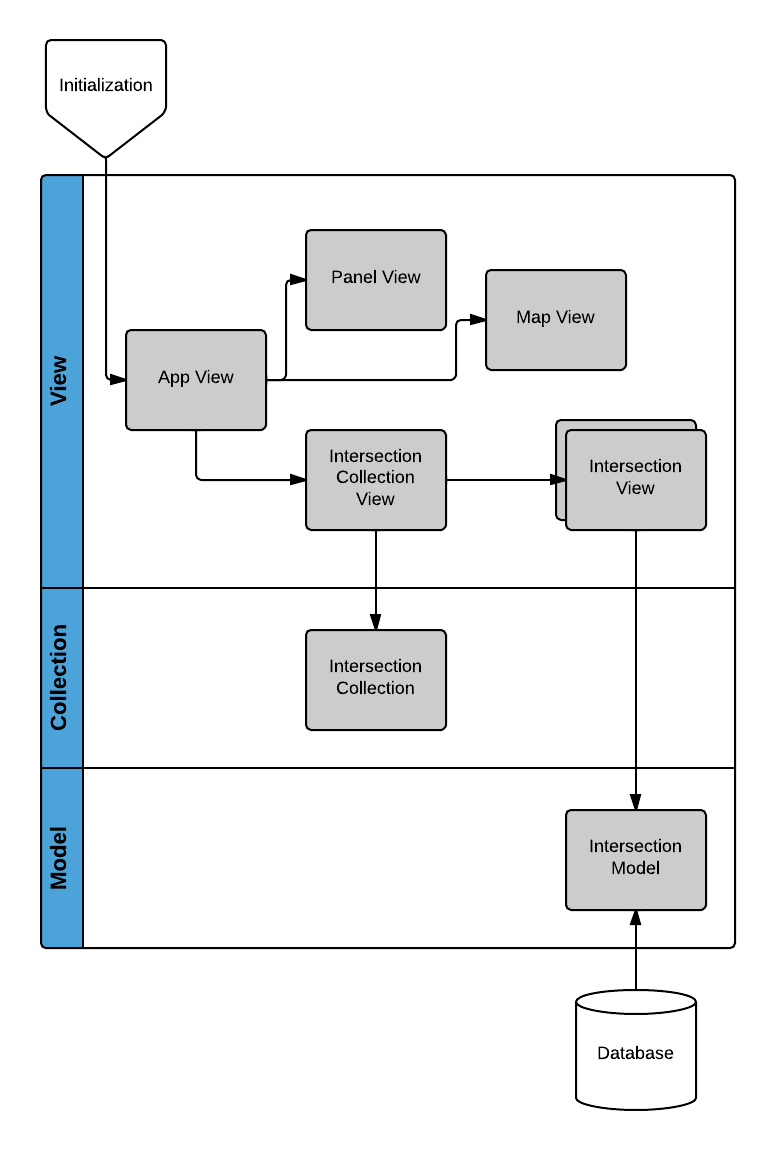
\includegraphics[scale=0.25]{figures/Iteration-2.png}
    \caption{An architectural diagram for Iteration 2.}
    \label{fig:iteration2}
  \end{centering}
\end{figure}

The third and final iteration of the architecture, as seen in figure \ref{fig:iteration3}, was developed for the final product demonstration and symposium. This architecture represents the full implementation as outlined and discussed within this report.

The overall structure of the application is similar to that in the second iteration. The App View class is responsible for the high-level initialization and management of the application instance. The App View also owns both the main model collections and page views. The Road Model, Road Collection, and associated views were added to support the display of road information within the interface. Furthermore, three new pages were added in addition to the original map page view: Intersections Page View, Roads Page View, and Network Page View. These pages utilize the exiting data, yet present fundamentally different views and functionality around the data, supporting many of the non-crucial functional requirements. The addition of non-page and non-model views, such as the Panel View and the Activity View, encourage the application of Backbone's MV framework for the sake of uniform code patterning.

The value of storing one instance of the intersection and road collection objects is now clear, as the four pages now feed off of the same two data representations. This also means that all updating and synchronization of information between the client and server has been centralized, and thus the data is guaranteed to be consistent across the application.



\begin{figure}[htbp!]
  \begin{centering}
    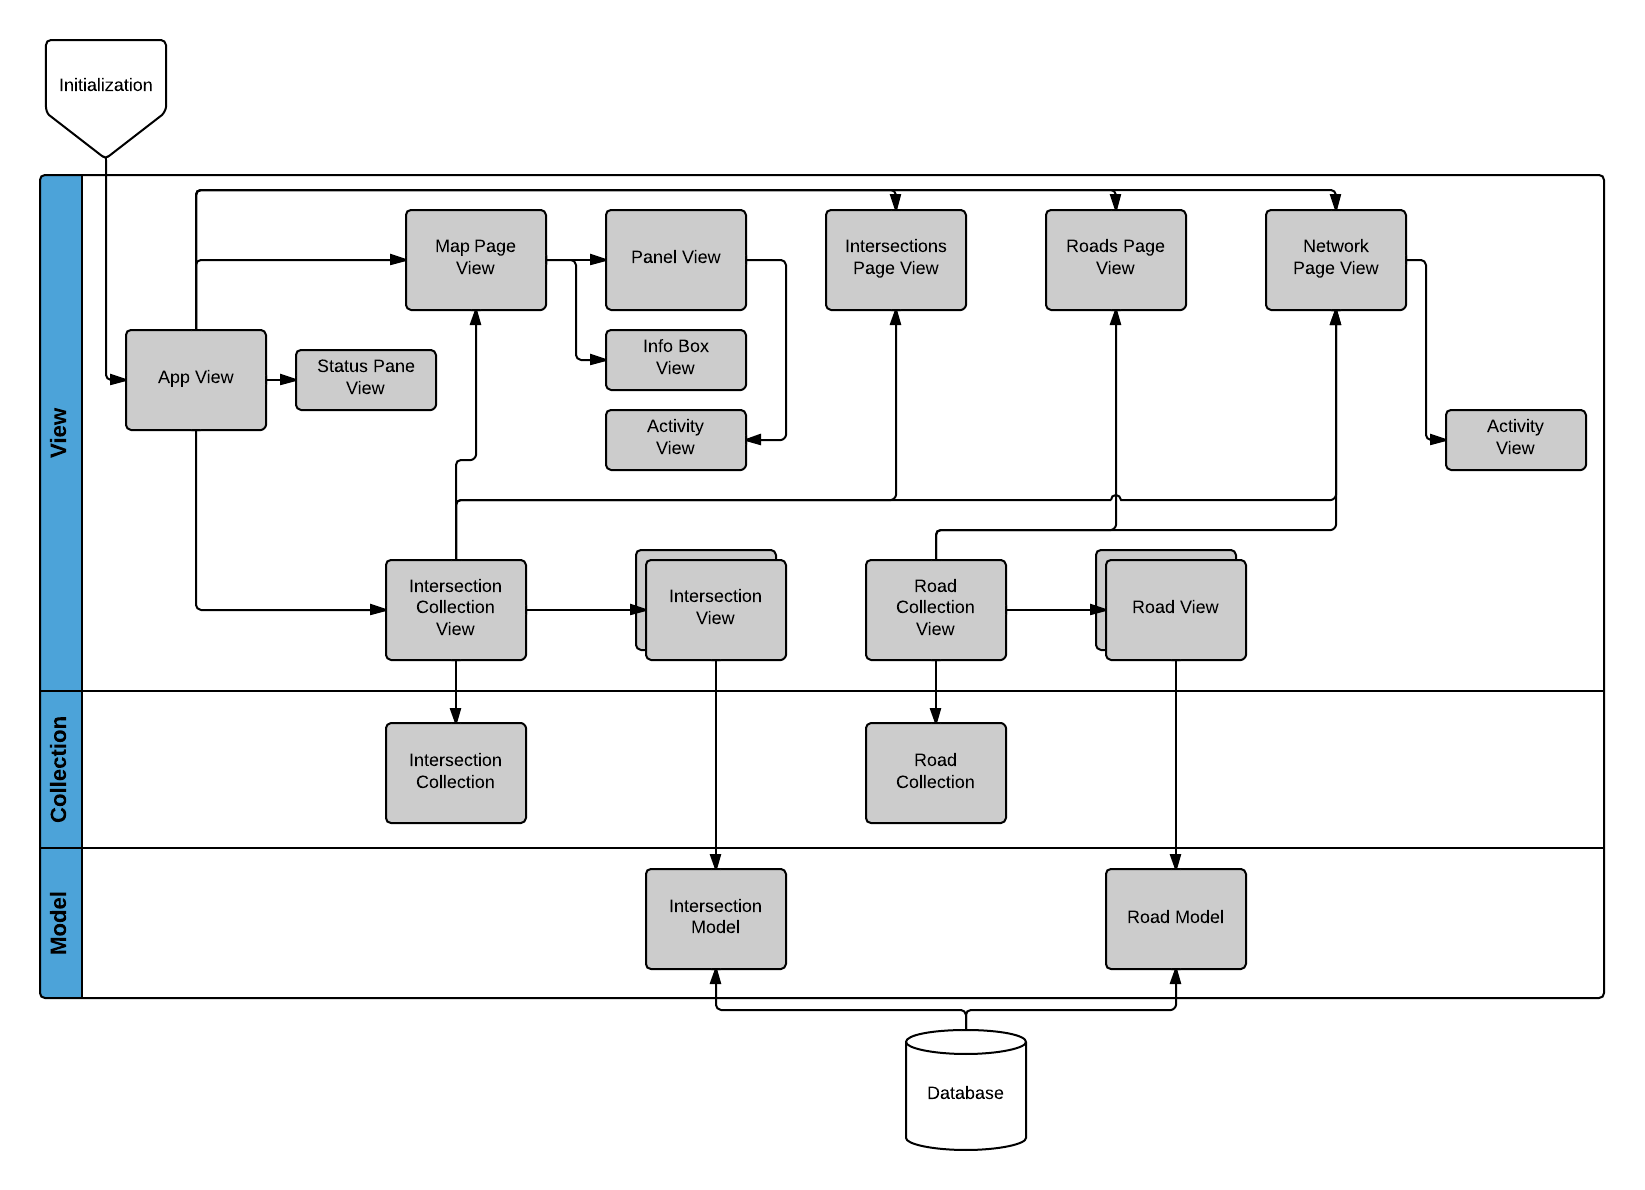
\includegraphics[scale=0.25]{figures/Iteration-3.png}
    \caption{An architectural diagram for Iteration 3.}
    \label{fig:iteration3}
  \end{centering}
\end{figure}

\section{Back End}
The infrastructure powering the user-facing component of Relay is colloquially referred to as the ``back-end''.
The design goal for this particular component consisted of providing all the necessary resources to the client-side application with minimal development effort (effort that would otherwise be spent on more innovative areas of development).
Additionally, this layer acts as the \emph{glue} that holds together the Relay system.
This is outlined at a high level in a full system map in Figure \ref{fig:Back_end_system_map}.
The back-end exposes APIs required for the client-side application (front-end), as well as data processing and scheduling routines for the Relay Framework.
This component is characterized by an application server, database, and associated services (such as map tiling).

The core application framework was chosen based on familiarity and flexibility (rather than performance).
For this task the ``Flask'' python framework was chosen, as many team members had worked in this environment successfully in previous projects.

\begin{figure}[H]
  \begin{centering}
    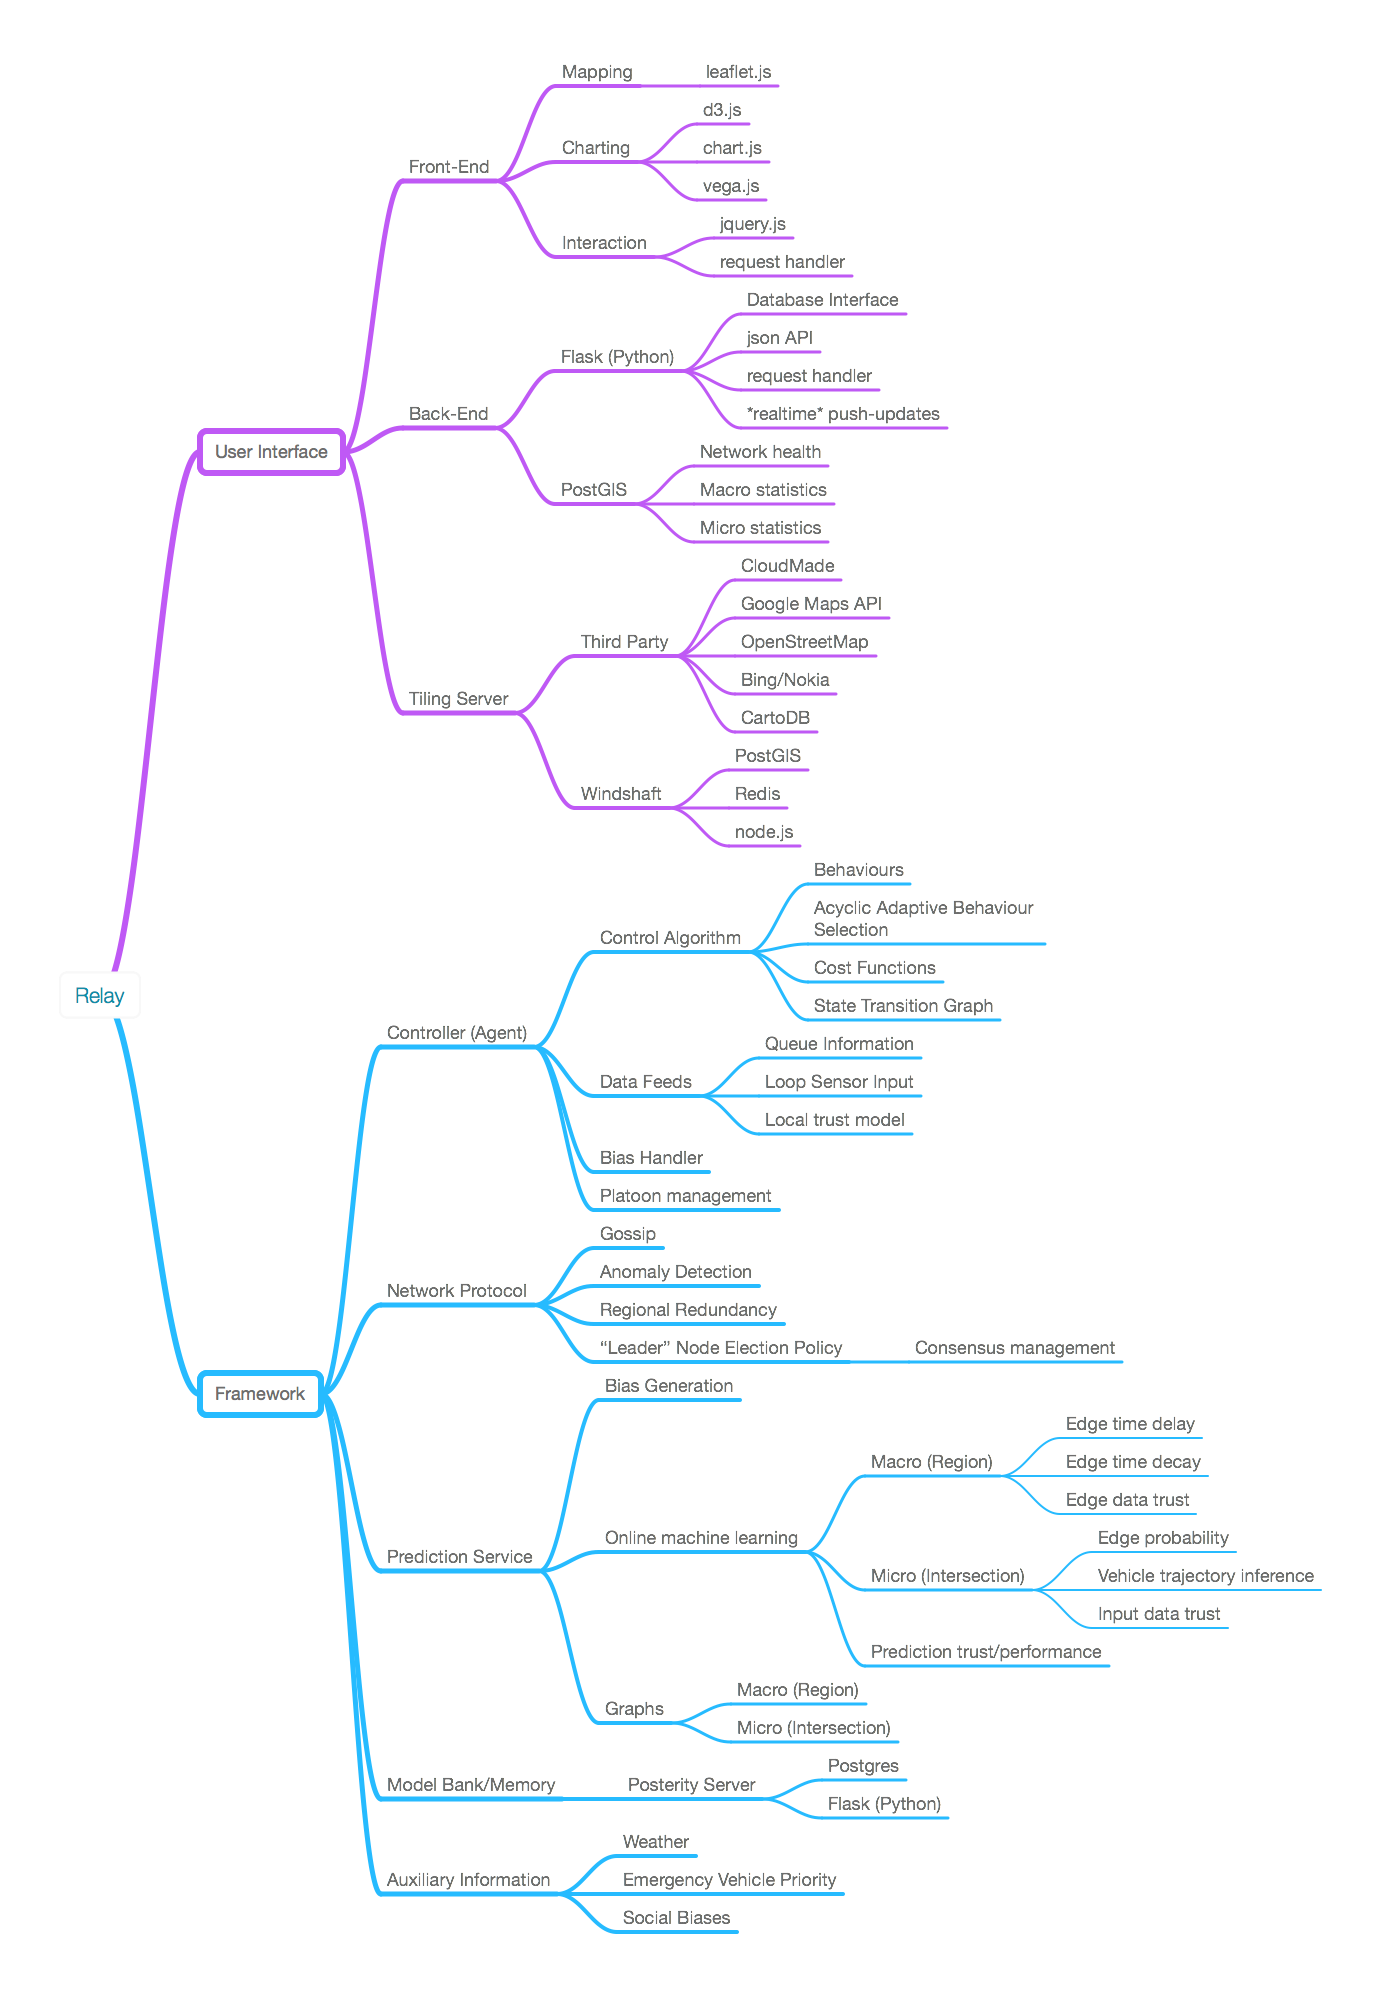
\includegraphics[scale=0.3]{figures/flow-chart.png}
    \caption{Relay: System Map}
    \label{fig:Back_end_system_map}
  \end{centering}
\end{figure}

Aside from the web-framework, the back-end design choices and technologies are broken up into modules.
To deliver the minimum viable product, the back-end must support online mapping via either a tile server or third party service, it must have some place to store various geospatial information (database), as well as some service to interface with the controller network (Relay Framework).
The various module design decisions and technologies selected are detailed below.

\subsection{Server - Flask and Python}
The Flask application acts a server with Relay passing information through the system to desired endpoints. This application contains functionality for transforming data, making network requests, serving information to front-end, and interacting with the database.

	Relay has multiple components and each works with the data in a specific format. Formatting is kept consistent throughout the system, using JSON formatted strings, but transformations are still required. The main transformation that needs to be performed is to change the time series data from the Erlang-server into information that can be better visualized on the front-end – explained in a <SECTION>.

	Network requests are defined by calls made to the Erlang-server, or “Framework”. The network contains all information regarding intersections, such as current behaviour, plans, and predictions. The Flask application is responsible for extracting this information and sending it to the database, front-end, or both.

	Lastly, the main function of the server is to accept requests from the front-end, process them, and serve the required information. Initially the majority of the information served comes from the database, but once the system is running, data is sent directly from the network to the front-end. This linkage is depicted in the system diagram, Figure \ref{fig:system-diagram}.

\subsection{Database - SQLite3}

As with most applications, the Relay web-service requires some medium to safely and efficiently store structured data, the canonical use case of a database.
Database technology is highly mature, and for its ease of use, familiarity, and extensive documentation, additionally, many members of the team are familiar with SQL.
To capitalize on this, a SQL relational database management system was chosen to power the Relay iInterface.

SQLite3 was chosen as the database for its simplicity. 
These databases are contained entirely within a single file, and as such can be quickly and easily moved around the development environment (as well as captured by version control). 
The database contains information for: road metrics, intersection metrics, events, and Toronto's intersections and roads, aquired from their public data website <TORONTO>.

'Road metrics' stores the time delay parameters for each segment, along with a timestamp and associated node ids at the ends of the segment. 
'Intersection status' contains the current status of each intersection. 
In the case of 'failure' states at any intersection, explainations and further information would be found in 'Intersection events'. 
Intersection behaviours and plans are not contained within the database as of this iteration. 
In the future they could be added for historical lookups and use in planning, but for the purposes of the prototype this feature was not included. 
Tables have been created for these and could easily be integrated into the system.

\begin{figure}[H]
  \begin{centering}
    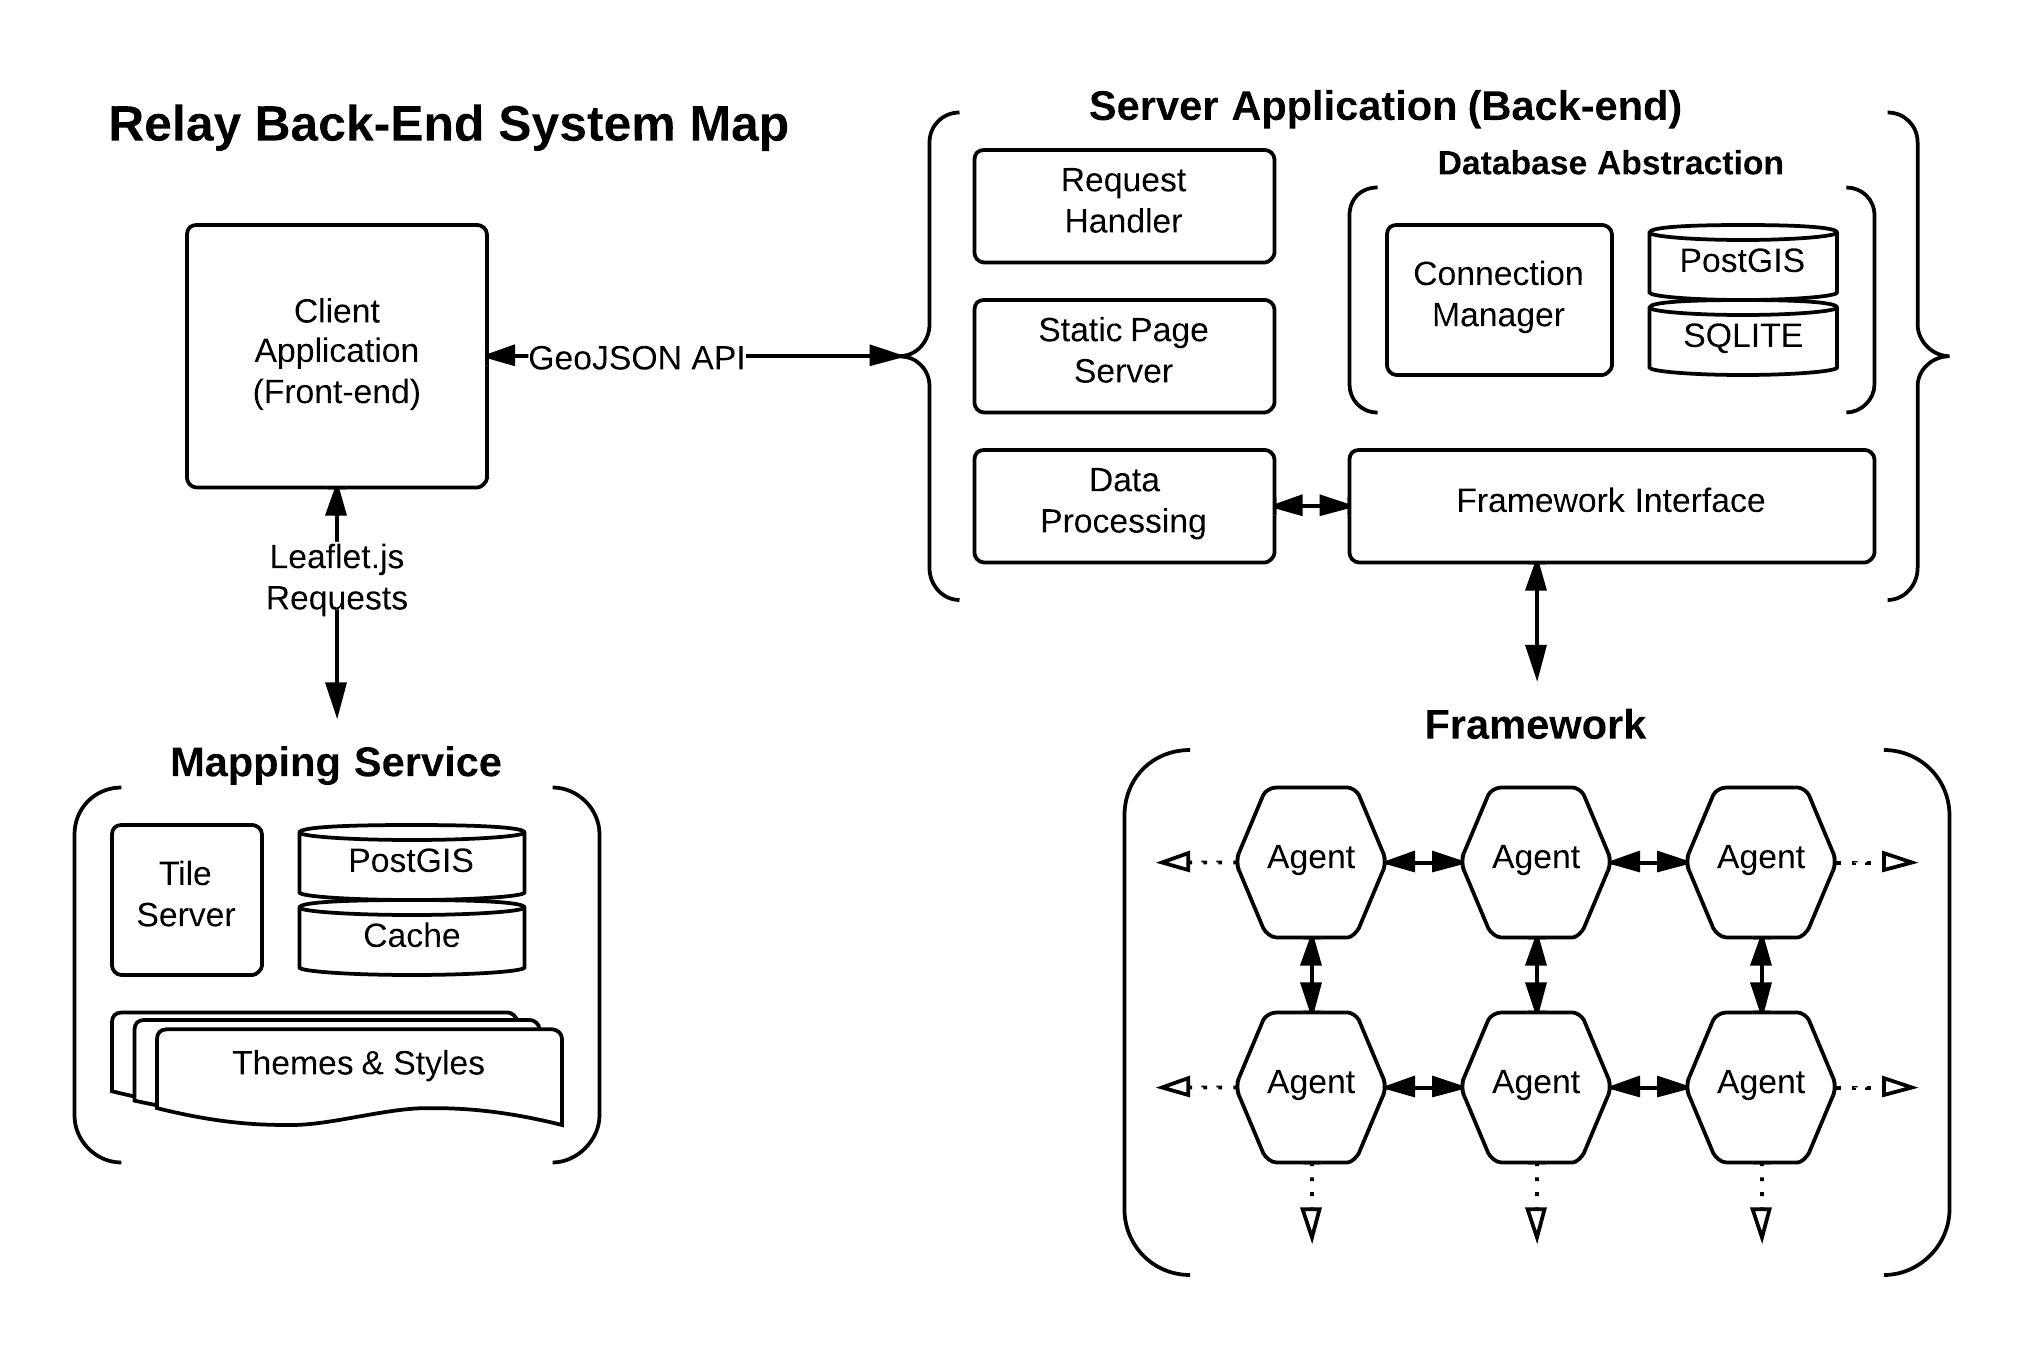
\includegraphics[scale=0.3,  angle=90]{figures/Relay_Backend_System_Diagram.png}
    \caption{Relay: Back-end System Diagram}
    \label{fig:system-diagram}
  \end{centering}
\end{figure}

\subsection{Client-Server Communication}
It is a goal of the solution to present up-to-date information about the network in the interface. This requires frequent communication between the client and the server. Client-server communication was achieved via the development of an Application Programming Interface (API) on the server, with which the client could connect to receive new information. The API was designed to specifically meet the needs of the solution, as API calls were designed specific features within the interface.

In order to maintain up-to-date information in the interface, the client was required to request new information from the API on a high-frequency schedule. Traditional HTTP requests require for the reload of a web page each time a request is made, so Ajax techniques were used in lieu of traditional HTTP requests. Ajax allows for asynchronous HTTP requests between the client and the server, which do not require the reload of the page upon completion. This successfully allowed for high frequency updates of the client without the negative performance implications of traditional HTTP calls.

\section{Deep End - Relay Framework}

Real-time, distributed traffic control is an interesting problem, with many creative solutions.
The modules and operators that handle individual intersection signal timing, data collection and backup, and statistical modelling, as well as the network topology that holds it all together is brought under the umbrella term ``Relay Framework''. \\

The goal of the framework is to address the intelligent traffic control problem from the \emph{bottom-up}.
Within the framework, each intersection is endowed with its own autonomous signal timing controller or ``Agent''.
In isolation, each Relay Agent seeks to maximize intersection throughput (as measured through various arbitrary metrics) subject to local environmental/contextual constraints. \\

\subsection{Architecture and Design}
\subsubsection{Relay Intersection Modelling}

In general, any intersection in Relay can be modelled as a graph (physically this is also the case).
Intersections in Relay are modelled as directed acyclic graphs, where each inlet and outlet are distinct nodes/vertices, and the edges are legal paths that a vehicle could follow to get from one inlet to a corresponding reachable outlet.
Each edge in the graph (aside from containing reachability/adjacency information) contains probabilistic information pertaining to that particular physical path.
This is shown in Figure \ref{fig:Relay_Intersection_Graph}.
At the highest level, the Relay Agent, in conjunction with its local prediction service learns a probability for each edge, which represents the liklihood that a vehicle will choose to traverse that given edge if it arrives at the originating inlet.
For example, in the case of an intersection with a dedicated left turn lane, the associated edge would have a probability of 1, meaning we would expect that all vehicles who enter the left-turn inlet, proceed to execute a left turn.
It also follows from this that the sum of out-going edge weights for a given inlet will always be one. \\

\begin{figure}[H]
	\caption{Relay Intersection Graph Model}
	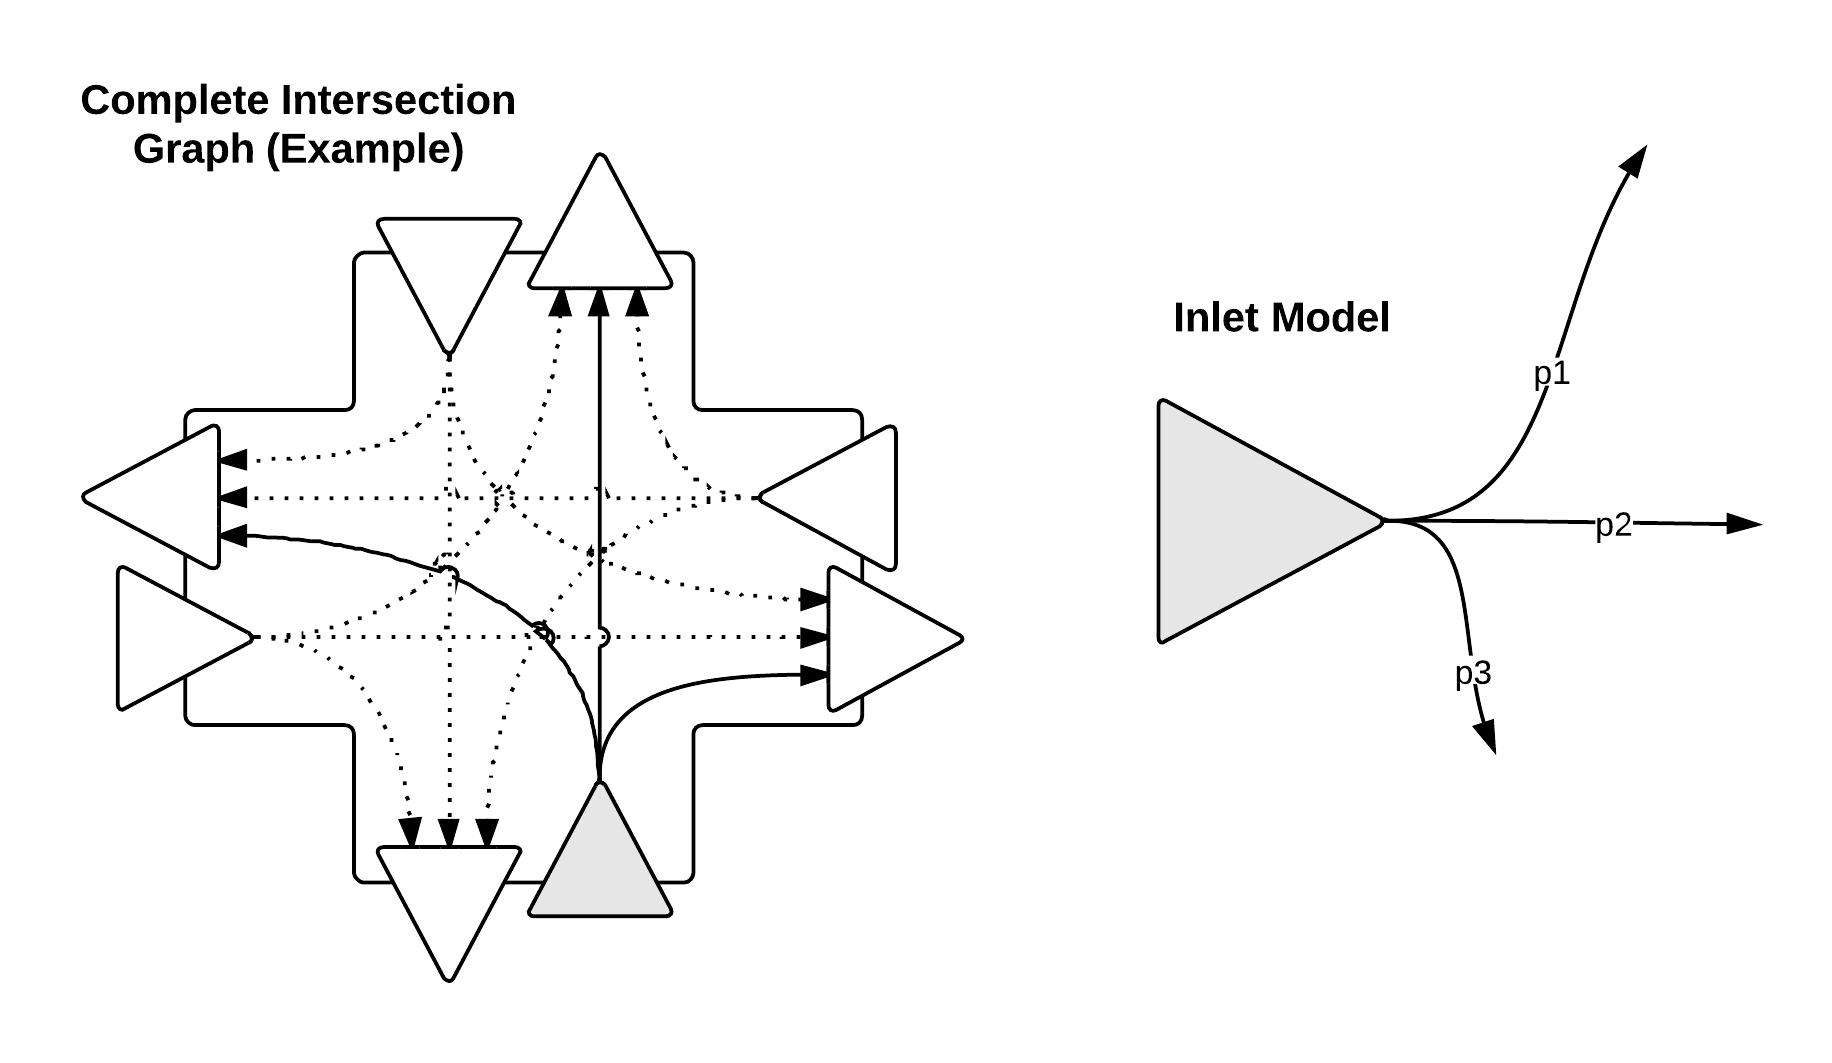
\includegraphics[width=\textwidth]{figures/Relay_Intersection_Graph.png}
	\label{fig:Relay_Intersection_Graph}
\end{figure}

Similar to the complete intersection graph, legal signal states (i.e. Green vs. Red lights) are also described as a graph.
These \emph{Behaviours} are subgraphs of the complete intersection graph, with similar properties.
Thus each behaviour describes a discrete number of inlets (and associated outbound edges) to serve at a given time, in this manner Behaviours can be chosen (by the controller) to serve the inlets that best maximize short-horizon flow.
Additional information regarding this process is discussed in the ``Relay Agent'' section below.\\

\subsubsection{Relay Agent}
The Agent module contains all the necessary ingredients for soft-real-time acyclic reactive adaptive signal timing.
An outline of the Agent module is contained in Figure \ref{fig:Relay_Agent_Controller}.
The controller is set up as a maximization process which weighs the current and predicted traffic profile (as well as queue statistics if they are available) and selects the appropriate \emph{behaviour} to optimally fulfill its objective function.\\

\begin{figure}[H]
	\caption{Relay Agent Controller}
	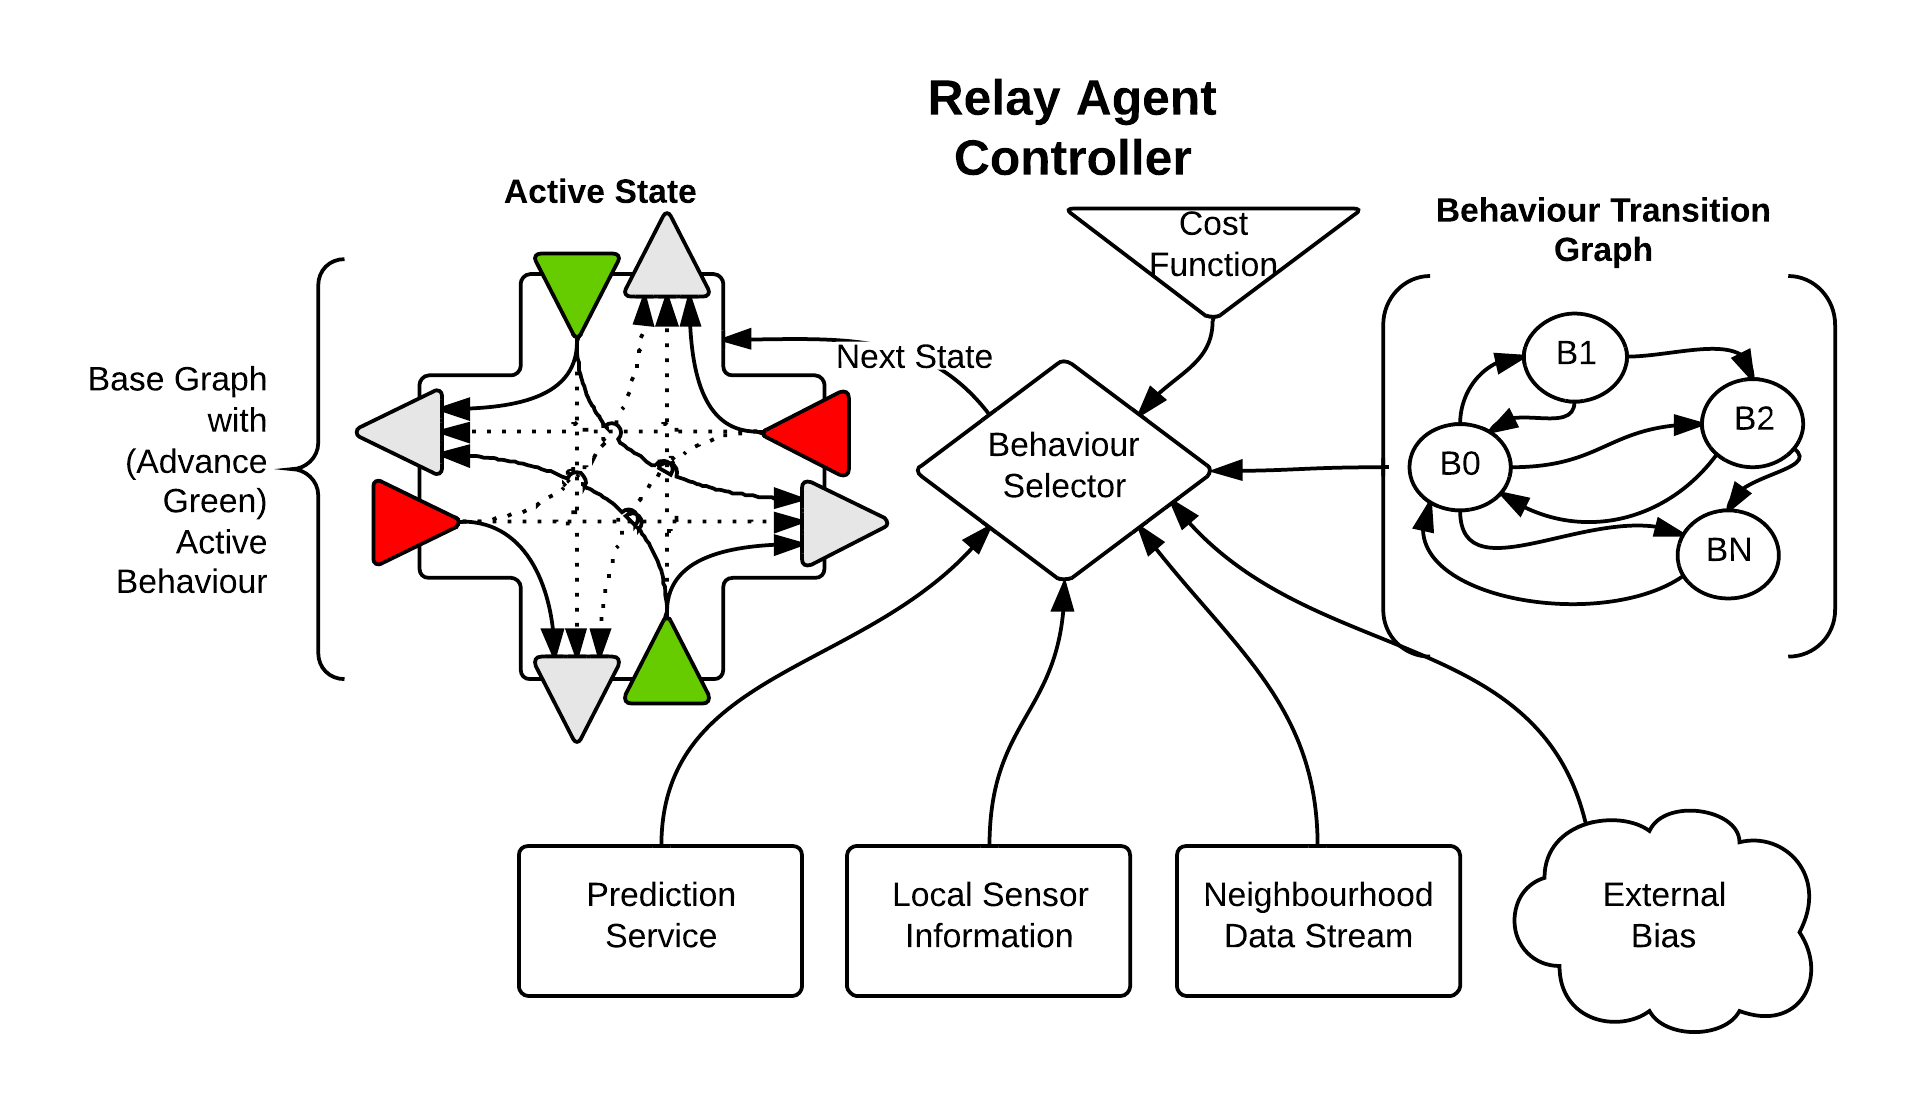
\includegraphics[width=\textwidth]{figures/Relay_Agent_Controller.png}
	\label{fig:Relay_Agent_Controller}
\end{figure}

Similar to the Relay Intersection model, the behaviour transition graph (or matrix, depending on the implementation) contains information related to the cost associated with changing the current signal, as well as logistic information such as minimum behaviour durations.
Where signal behaviours are encoded as nodes/vertices, transition costs (dead time, minimum signal duration, vehicle lag, etc.) are among the edge properties. \\

For example, switching the direction of traffic flow cannot be done instantaneously, furthermore in most countries there is a minimum amount of ``red'' time that must be allocated in both directions to allow lagging traffic to safely exit the intersection.
Thus the amount of time required to switch a particular signal behaviour depends on the current state of the intersection.
As another example, consider the concept of an \emph{advance-green} a behaviour typically following ``red''-time favouring a particular direction, granting vehicles wishing to turn left right of way for an arbitrary amount of time.
In Relay, this advance green signal is treated no differently from any other signal behaviour.
In this case the associated transition cost to switch behaviours from advance green to \emph{full} green is very low.
This information is encoded in the edges of the behaviour transition graph. \\

Aside from dictating the signal behaviours and durations, the Agent is also responsible for updating its internal intersection probabilities, and processing/interpreting local traffic sensor data.
It is important that in the scope of this project, we have assumed we have \emph{perfect} traffic data at the intersection level.
We acknowledge that this is a large assumption that is not necessarily realistic most traffic systems have notoriously poor sensing capabilities \cite{Miovision:2012}.
However as a matter of scope, many companies (such as the Kitchener-based Miovision) have commercial solutions to this problem.
As a coping mechanism, it may be possible to leverage the Relay prediction service to develop an internal \emph{trust} model associated with each intersection's sensors.\\

\subsubsection{Network Topology}
\label{subsubsec:net-top}

To a particular Agent, the Relay Framework appears as a mesh network centred around it.
The choice of network topology was not difficult given our design constraints (for the Framework) include a high degree of fault tolerance, robustness, and physical distribution.
Peer-to-peer (p2p) Mesh network topology (aside from being relatively novel) is a natural fit for these kinds of constraints.
Particularly as many of the technology's weaknesses (poor latency, poor scaling behaviour for complete connectivity of all Agents, etc.) are explicitly avoided by the Relay Framework Architecture.\\

In traditional Mesh Networks, each node is tasked with repeating the messages of other nodes to its neighbours/peers.
This results in a lot of overhead for individual nodes.
Within the Relay Framework, Intersection Agents do not require an active connection to every other Agent in the network, they only care about their immediate (or to some finite-depth) neighbours.
This depth-wise priority is shown in Figure \ref{fig:Relay_Network}.\\

\begin{figure}[!htpb]
	\caption{Relay Network Neighbourhood}
	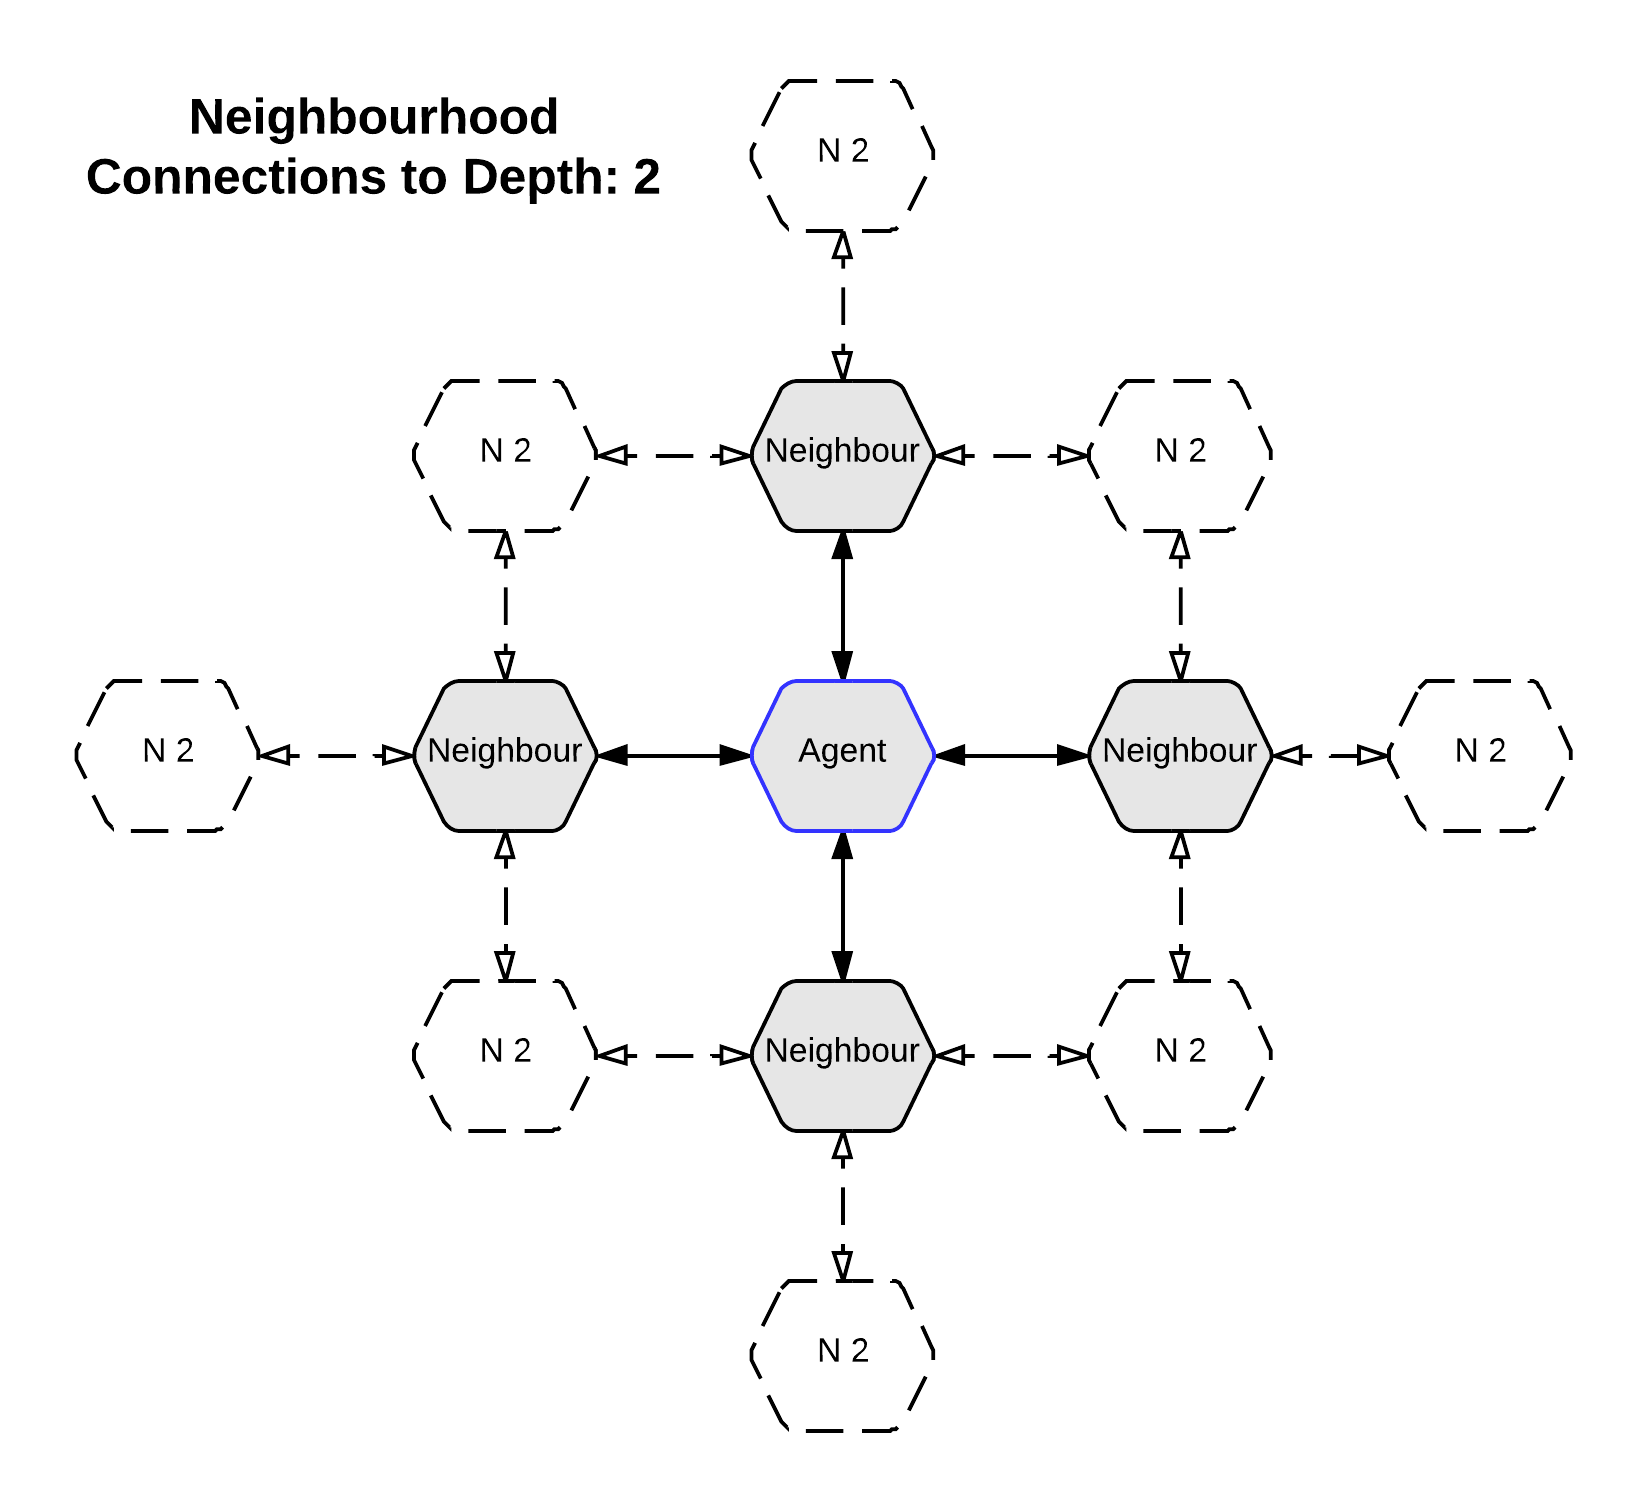
\includegraphics[width=\textwidth]{figures/Relay_Network.png}
	\label{fig:Relay_Network}
\end{figure}

Alternative network topologies have been used by current adaptive traffic implementations.
For small scale (arterial) installations, it is trivial to have all agents permanently connected to all peers.
Modern installations have also implemented so-called ``cloud-service'' based approaches, and Miovision's Spectrum is one such example.\\

\subsection{Learning in Relay}
\subsubsection{Design Parameter Updates}

Each agent within the system has multiple design parameters that will constantly update. With each cycle -- behaviour change -- predictions and estimations are made to recalculate these parameters. 
The following sections explain how these variables are learned and updated.

\subsubsection{Time Delay Estimation}
The first important parameter needed to calculate predictions is the time delay estimate between two agents. 
This can be thought of as the estimated time to travel from one intersection to a neighbouring one. 
However, this is not a fixed time, so the delay is modelled using a gamma distribution, as discussed previously. 

The first step in performing this estimation, is determining which portion of the downstream signal is relevant – meaning what part of the signal should be considered for the estimation. 
This is required because it must match the departing signal from the upstream intersection. 
To extract the downstream signal, an upstream sub-signal is first selected. It was determined that the most efficient way to do this is to this is to select the upstream departure signal created by the previous behaviour cycle. 
To ensure that events are not missed, the downstream signal is determined by time-shifting the upstream signal by the expected value of the previous time delay distribution, and a small buffer is added to each end.

After the two signals are extracted, the estimation process can be performed. 
Equation [time-delay-opt] outlines the optimization problem, using least squares. 
The goal of this optimization is to convolve the departure signal with a gamma distribution to best estimate the downstream arrival signal -- to minimize the difference between the real signal and estimated. 
The design parameters are: shape, location, scale, and gain. 
The first three are what control the parameters of the distribution and the last is a measure of the change in cars while traversing the road -- to capture the effect of cars turning onto or off of the road on side streets.

Below, in Figure \ref{fig:time-delay-est}, an example estimate is performed. 
Two signals are provided (departure is pre-calculated within the agent and not shown here), trimmed, and then the optimization procedure is executed. 
The resulting distribution is overlaid on the downstream signal and estimated time delay gamma plotted above.

\begin{figure}[H]
  \begin{centering}
    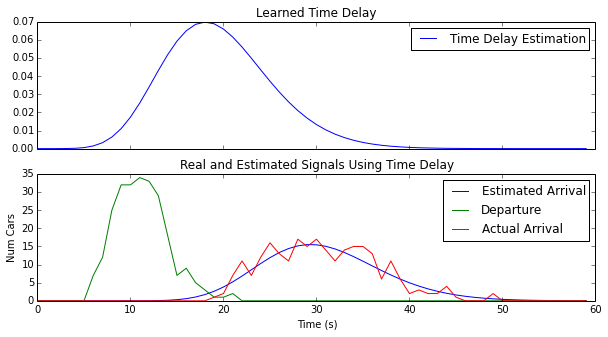
\includegraphics[scale=0.75]{figures/time-delay-est.png}
    \caption{Example time delay estimation.}
    \label{fig:time-delay-est}
  \end{centering}
\end{figure}


\subsubsection{Updating Intra-Agent Behaviour Graphs}
The second important piece in generating signal predictions is learning the intra-agent graph probabilities. 
These represent the likelihood of a signal to travel along this edge during the executed behaviours cycle.

\paragraph{Behaviour Probability Matrix (BPM)}
Figure \ref{fig:BPM-example} provides a visualization of this to help parse this idea. 
The matrix represents how these edge probabilities are used within the system; in the matrix, departing nodes are along the columns and entering along the rows -- $p_{02}$ would represent entering node 0 and exiting node 2. 
It is seen in the diagram that an event occurring at node 0 has a 60\% likelihood of exiting node 2, for this behaviour.
 It is important to not that edges that are not traversable will always have a probability of 0. 
Essentially, this probability matrix is used to split an entering signal into components, to then be combined with other estimates in a departing signal. 
This estimated signal is then used in combination with the time delay estimation to predict expected traffic, which will be discussed further in the following section.

\begin{figure}[H]
  \begin{centering}
    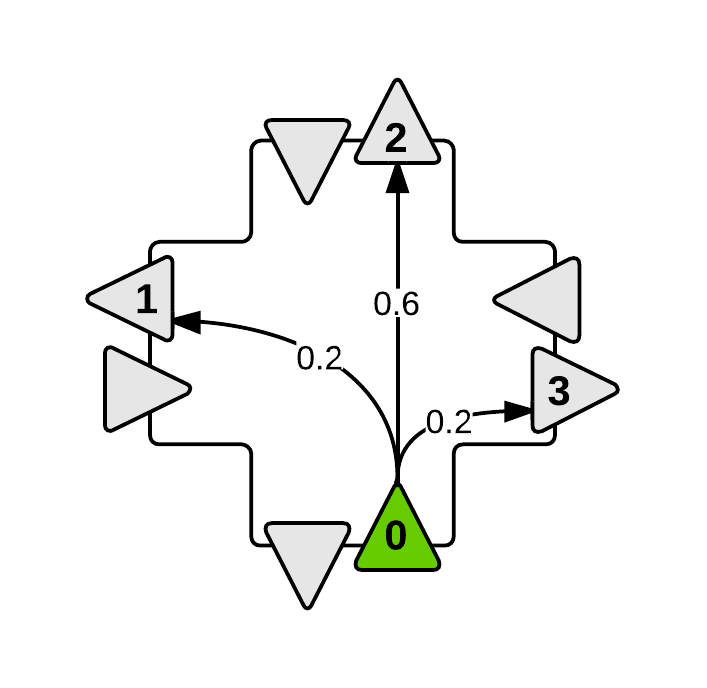
\includegraphics[scale=0.3]{figures/BPM-example.png}
    \caption{Example intra-agent edge probabilities for node 0.}
    \label{fig:BPM-example}
  \end{centering}
\end{figure}


\[
{BPM} =
    \begin{bmatrix}
    p_{00} & p_{01} & p_{02} & p_{03} \\
    p_{10} & p_{11} & p_{12} & p_{13} \\
p_{20} & p_{21} & p_{22} & p_{23} \\
p_{30} & p_{31} & p_{32} & p_{33} \\
    \end{bmatrix}
\]

\paragraph{Learning Probabilities}
This is an extremely challenging multi-objective optimization problem and multiple approaches were taken to try to solve it. 
As with the time delay estimation, this is essentially a least squares problem, but much more complex. Equation \eqref{eqn:bhvr-opt} outlines the optimization procedure.  \\

\begin{equation*}
\label{eqn:bhvr-opt}
\begin{aligned}
& \text{minimize}
& & \sum_{j=0}^{3}\sum_{k=0}^{n} \left \| d_{kj} - \sum_{i=0}^{3}(p_{ij} \times c_{ki}) \ast \tau_j \right \| \\
& \text{subject to}\\
& & \sum_{i=0}^{3} P_{ij} = 1 \\
& & p_{i=j} = 0 \\
& & 0 \leq p_{i\neq j} \leq 1
\end{aligned}
\end{equation*}
Where:
\begin{conditions*}
j & outlet node \\
i & inlet node \\
k & index in sampled signal \\
d_{kj} & $k^{th}$ element in downstream neighbour arrival signal connected to agent node $j$ \\
c_{ki} & $k^{th}$ element in inlet signal at agent node $i$ \\
p_{ij} & corresponding inlet-outlet edge probability \\
\tau_{j} & time delay distribution along edge connecting agent node $j$ to neighbor \\
\end{conditions*}

This is an underdetermined system and thus cannot be solved with normal optimization methods, as is. 
The first alternative method attempted was reinforcement learning (RL).
 RL attempts to punish or reward actions for their ability to reach a desired outcome. 
In this problem, edges would be rewarded when their estimated signal closely matched a portion of the real downstream signal. 
Conversely, they would be punished when the estimated signal, over- or under-estimated the downstream one. When investigated further it was determined that this problem does not quite fit the requirements for an RL implementation and would be difficult to transform this into something that could work with existing python RL libraries (e.g. PyBrain). \\

Next, reducing the number of design parameters was investigated. 
For a given behaviour, some edge probabilities will always be 0 – these edges are not allowed paths – and therefore these could be removed and the problem space reduced. 
This method was determined to be infeasible due to the fact that a customized optimization procedure would need to be written for each possible behaviour – the Python implementation for optimization requires that constraints be explicitly written for the procedure to work. 
Running the procedure without constraints was tested, but this failed as invalid edge probabilities were found (i.e. greater than 1 or less than 0), as expected. \\

Thirdly, attempting to solve the problem with a linear least squares regression model ($Ax=b$) was performed. 
The signals were taken into Fourier space to remove convolution from the equation, and parameters solved. 
The $A$ matrix in this formulation is unknown and represents the behaviour probability matrix. 
It was isolated and solved for with the formulation: \\

\begin{align}
	A& = DX^{T}M \\
	M& = (X^{T}X)^{+} \\
	X& = C \ast \tau
\end{align}
Where:
\begin{conditions*}
D & vector of neighbor departing signals \\
C & vector of arrival signals
\end{conditions*}

This formulation was tested and found to not produce useable results. 
Again, probabilities were found that did not fit within the required constraints.\\

\paragraph{Updating BPMs}
After the optimization procedure has arrived at a solution, the existing BPM must be updated. 
It would be unwise to directly use the newly calculated BPM as temporary inhibitors to traffic flow, such as accidents, can greatly skew results. 
Therefore, a learning parameter is used to update existing probabilities, seen in Equation \eqref{eqn:BPM-update}. 
This can be tuned, on an agent-by-agent basis, to alter how quickly these values are modified and adapt – an average of the two values is a good starting point, to enable quick transitions, while remaining relatively stable. 
In \eqref{eqn:BPM-update}, $i$ represents the agents ID and $BPM_{est}^{i}$ is the newly estimated behaviour probability matrix for that agent.

\begin{equation}
    BPM_{new}^{i} = \alpha^{i} \times BPM_{old}^{i} + (1 - \alpha^{i}) \times BPM_{est}^{i}
    \label{eqn:BPM-update}
\end{equation}

\subsection{Predictions in Relay}
Making predictions of traffic is an essential component of Relay. 
This is the foundation of intelligence in the system and assists each agent in making decisions regarding behaviour execution. 
Predictions represent an estimation of local traffic $x$ seconds into the future, with the length being determined by the needs of the controller. 
Higher-order predictions, one’s that require information from the larger neighborhood, can also be generated, but with less fidelity. 
The details on how these predictions are performed is discussed below.

\subsubsection{Utilizing Neighborhood Information}
As discussed in section~\ref{subsubsec:net-top}, agents are connected to each of their neighbors, forming a grid-like mesh structure. 
This design choice allows for each agent to ``talk” with its neighbors, gaining access to all information stored. 
This ``sharing” of information is essential to keep agents informed on events occurring in the neighborhood.
Information is either requested or directly sent to a specific agent, depending on the type: current queues, predictions, plans, events, etc.
 Agents can freely communicate by simply ``asking” their neighbors for the specified data. 
An event centre is constructed on each agent to handle incoming and outgoing requests, making communication efficient and standardized across the network (discussed further in later sections). \\

	While an agent is not directly connected to other agents in its extended neighborhood, if required, it can indirectly access this information. 
Any agent can ``inject" requests into its neighbors to obtain information from their neighbors, and so on (again, specifics discussed in later sections). 
This isn’t used often, as fidelity decreases quickly as requests propagate outward, but, for example, it is necessary for calculating higher-order predictions. \\


\subsubsection{Making a Prediction}
To make a prediction, the agent must combine the learned edge probabilities with the time delay estimates for each neighboring agent. 
This utilizes previously calculated information about the agent’s in the neighborhood, to derive a predicted incoming signal for each node at the agent of interest. 
Equation \ref{eqn:first-order-pred} outlines the basic formulation for making this prediction, $Pr_{i}$, where $i$ represents the inlet node id. 
If the length of signal initially calculated is longer than the requested time, excess information will be trimmed. 
If the length requested is longer than this next-neighbor prediction, a higher-order prediction is calculated, known as $Pr_{i}^{*}$.\\

This information also creates useful visualizations for traffic engineers, giving them the ability to ``see into the future”. 
While they wouldn’t necessarily act upon this information, they would have an expectation of traffic at each intersection. 
It also gives context for why the next behaviour was selected (i.e. the ``plan") – this is discussed further in later sections.\\

\begin{equation}
	Pr_{i}^{\star} = d_{e_i} \ast \tau_{i}
	\label{eqn:first-order-pred}
\end{equation}
\begin{equation}
	d_{e_i} = \sum_{k=0}^{3} p_{kj}^{nbr} \times c_{k,i}^{nbr}
	\label{eqn:first-order-d}
\end{equation}
Where:
\begin{conditions*}
p_{kj}^{nbr} & edge probability for signal at $k^{th}$ neighbor node, exiting $j^{th}$ node \\
d_{e_i} & expected departing signal from neigbhor node connected to agent node $i$ \\
c_{k,i}^{nbr} & real incoming signal at $k^{th}$ node of neighbor agent connected to agent node $i$ \\
\tau_{i} & time delay distribution along edge connecting agent node $i$ to neighbor \\
k & neighbor inlet id \\
j & neighbor outlet id
\end{conditions*}


\subsubsection{Higher-Order Predictions}
As mentioned previously, if the requested prediction is longer than the neighbors can provide, a higher-order, or remote, prediction is made. 
This is performed in the same manner as a first-order prediction, but utilizes each neighbor’s current incoming prediction signal as well, $Pr_{k,i}^{nbr}$.
 If even larger predictions are required, predictions can be extended to more distant nodes, but these would be very low quality and carry low weight – these are multiplied by each intersections edge probability, intrinsically lowering their strength. 
Again, the signal is trimmed at the end to match the requested length.\\

\begin{equation}
	Pr_{i} = d_{e_i} \ast \tau_{i}
	\label{eqn:higher-order-pred}
\end{equation}
\begin{equation}
	d_{e_i} = \sum_{k=0}^{3} (p_{kj}^{nbr} + Pr_{k,i}^{nbr}) \times c_{k,i}^{nbr}
	\label{eqn:higher-order-d}
\end{equation}
Where:
\begin{conditions*}
Pr_{k,i}^{nbr} & prediction signal at $k^{th}$ neighbor node, connected to agent node $i$ \\
p_{kj}^{nbr} & edge probability for signal at $k^{th}$ neighbor node, exiting $j^{th} $node \\
d_{e_i} & expected departing signal from neigbhor node connected to agent node $i$ \\
c_{k,i}^{nbr} & real incoming signal at $k^{th}$ node of neighbor agent connected to agent node $i$ \\
\tau_{i} & time delay estimation along edge connecting agent node $i$ to neighbor \\
k & neighbor inlet id \\
j & neighbor outlet id
\end{conditions*}

\newpage
\chapter{Design Testing and Validation}

\section{Front End}

\section{Back End}
As the intermediate layer between the Relay Framework, and the Relay Interface, the back-end performs little in the way of computation (other than ETL associated with communication).
Thus the main requirement is to respond to requests from the Relay Interface promptly.
Noticeable lag between modules, especially as it relates to the interface can dramatically reduce the end-user experience.
While this may not be of paramount importance for prototyping, it does become useful during development, and is further exacerbated by our technological constraints (hosting the platform locally on our personal computers).

That said, within the realm of software development there are a large battery of tests/testing-related-philosophies that could see application within this project.
At the highest level, system integration tests will be used to ensure platform robustness, especially in development.
At the code module level, the typical suite of unit tests will be used to assert correctness.
However, due to time requirements, rigorous testing is neither wanted nor warranted, and as such only the most critical systems will be tested in this way.
For example, the request handler is invoked every time the Interface needs new information, this module should be exceptionally robust to failure.
In a similar fashion, database connections can involve a significant amount of complexity if handled poorly.
Within this respect we follow the motto that the architecture should guide development to reduce the likelihood of system failure.
In this string, we have endeavoured to architect the Relay system as multiple pseudo-independent modules, each with their own functional (correct) core.
This design pattern is commonly referred to as ``Ports and Adapters'' or ``Hexagonal Architecture''.

\section{Deep End}

\newpage
\chapter{Recommended Design Modifications}

\section{Front End}

\section{Back End}

\section{Deep End}

\newpage
\chapter{Timeline and Project Management}

\section{Tasks and Deliverables}

\subsection{Fall 2013}
Below is an overview of the tasks to be completed over the Fall 2013 term. 
These outline the major milestones and steps that will be taken to create the first prototype, presented at the end of this term. 
The description column goes into detail about what will be performed in this task, and in many cases describes what will be included in that tasks deliverable. 
The deliverable column, where applicable, identifies the high-level product of each specific task.
\\

\begin{longtable}[htbp] {| P{2.5cm} | P{10cm} | P{2.5cm} |}
    \hline
    Task                                       & Description                                                                                                                                                                                                                                                                                                                                                                                & Deliverable                                        \\ \hline
    Idea Generation (W0-W1)                    & Researched existing solutions that attempt to tackle the problem or interest, or something similar. Brainstormed ideas and identified shortcomings of existing products to determine specifications and features of our proposed solution. Researched applicable technologies that will be potentially useful in building solution. Met with supervisor to gain initial thoughts. & N/A                                                \\ \hline
    Design Proposal (Oct 11)                   & Outlining and detailing the proposed design project idea. State of the art, needs analysis, and design specifications and requirements are provided.                                                                                                                                                                                                                                       & Report                                             \\ \hline
    Gain Supervisor Insight (W2)               & Meet again with supervisor to discuss our proposed idea and plan. Get his insight on our solution/plan/etc. and input on what we could change or improve.                                                                                                                                                                                                                                  & Copy of Design Proposal                            \\ \hline
    Design Proposal Presentation (W2)          & Presentation of project proposal. Summarize contents of report and gain feedback from classmates on idea. This will be a project `defence' and will also gain feedback from MBET students.                                                                                                                                                                                                 & Presentation and slides                            \\ \hline
    Design Critique/ Feedback (W2)             & Submit an assessment for two other projects both during presentation and prototype demo.                                                                                                                                                                                                                                                                                                   & Report                                             \\ \hline
    Low-fidelity Simulation Design (W3)        & Based on proposal, begin designing simulation environment for underlying system. This will be a set of wireframes and sketches of the final product. The team will discuss and iterate on these until a final design is chosen.                                                                                                                                                             & Wireframes and sketches of proposed solution       \\ \hline
    Early System Architecture (W3)             & Based on proposal begin designing and further researching each of the initial ideas. Obtain better understanding of what will be required to be developed (e.g. intersection network). Decide what technology will be used (e.g. CartoDB).                                                                                                                                                 & System architecture design and required technology \\ \hline
    Ongoing Research and Learning (W3 - W5)    & Perform further research on technologies and knowledge required to construct system. Will need to learn concepts in: machine learning, neural networks, network programming, distributed systems, and simulating these types of systems.                                                                                                                                                   & N/A                                                \\ \hline
    Update Meeting (W3/4)                      & Meet with supervisor to discuss current progress. Bring up any difficulties we are having and work through these.                                                                                                                                                                                                                                                                          & N/A                                                \\ \hline
    Mid-Fidelity Design (W3 - W4)              & Basic Quartz Composer mock-up created. This will have interactions developed and will allow us to iterate and improve the simulation environment.                                                                                                                                                                                                                                          & Quartz Composer mock-up                            \\ \hline
    Mid-Fidelity System Architecture (W4 - W6) & Designing functionality of ``actors'' (i.e. intersections). Begin development of network architecture (how do you connect all actors together?). Further research of programming paradigms required to construct the system.                                                                                                                                                                 & Architecture designs                               \\ \hline
    High-Fidelity Simulation Design (W6)       & High quality quartz composer mock-up. Have all basic functionality designed and prototyped. UI assets designed/created.                                                                                                                                                                                                                                                                    & Quartz-Composer mock-up                            \\ \hline
    Initial System Development (W6 - W7)       & Begin construction of system: ``agents'', ``network'' components, application infrastructure. Begin designing/building interfaces with sim-env.                                                                                                                                                                                                                                                & N/A                                                \\ \hline
    Sim-env Dev (W7-W8)                        & Begin developing the simulation environment. Create basic features.                                                                                                                                                                                                                                                                                                                        & Passes unit tests                                  \\ \hline
    Finish Prototype System Dev (W7-W8)        & Ability to set-up a network of actors, actor functionality established, and actors able to `talk' to each other.                                                                                                                                                                                                                                                                           & Passes unit tests                                  \\ \hline
    Simulation and System Testing (W8-W9)      & Testing of sim-env and system for prototype demo. Fix any issues that arise.                                                                                                                                                                                                                                                                                                               & Passes unit tests                                  \\ \hline
    Design Critique (TBD)                      & This will be a presentation to a group of ``Dragon's''. Similar to design proposal presentation and group will defend the proposed idea and solution. Will go in depth in how the solution is superior to current state of art.                                                                                                                                                              & Presentation and slides                            \\ \hline
    Prototype Demo (Nov 29)                    & First demo of project. Team will present the first prototype that has been created. Will identify challenges that arose, what modifications needed to be made, and what the next steps will be to reach end goal.                                                                                                                                                                          & Presentation, demo, and slides                     \\ \hline
    Design Brief (Dec 7)                       & ~        Summary of progress this term.                                                                                                                                                                                                                                                                                                                                                                                   & ~           Report                                       \\ \hline
    Outreach Presentation (TBD)                & Participate in UW sponsored event to demonstrate project. Will be used to showcase SYDE design projects and gain outside feedback on our project.                                                                                                                                                                                                                                          & ~                     Presentation, summary.                             \\ \hline

\end{longtable}

\subsection{Winter 2014}
Below is an overview of the tasks to be completed over the Winter 2014 term.
These outline the major milestones and steps that will be taken to create the final prototype, presented at the final symposium.
The description column goes into detail about what will be performed in this task, and in many cases describes what will be included in that tasks deliverable.
The deliverable column, where applicable, identifies the high-level product of each specific task.\\

\begin{longtable}{|p{4.5cm}|p{6cm}|p{4.5cm}|} \hline
    Task                                              & Description                                                                                                & Deliverable                           \\ \hline
    Team Debrief, Update (W1)                         & After the Holiday's team will meet over the first few weeks to get back up to speed with what was accomplished the previous term and over the break as well. Will begin creating a detailed list of tasks to be completed.         & N/A                                   \\ \hline
    Response to Feedback (Jan 21)                     & Details of this report TBD                                                                                                                                                                                                         & Report                                \\ \hline
    Meet with Supervisor (W2)                         & Meet again with supervisor to discuss our progress and plan. Get his insight on our solution/plan/etc. and input on what we could change or improve.                                                                               & N/A                                   \\ \hline
    Actor Development and Research (W2)               & Continue building functionality of ``actors'' (i.e. intersections). Begin development of network architecture (how do you connect all actors together?). Further research of programming paradigms required to construct the system. & Architecture designs and construction \\ \hline
    Application Development (W2)                      & Continue iterating on current interface/interaction design. Add more features (e.g. advanced traffic information panel) and incorporate newest functionality from back-end.                                                        & Updated interfaces and application    \\ \hline
    Network Development (W3-W4)                       & Ability to set-up a network of actors, actor functionality established, and actors able to ?talk? to each other.                                                                                                                   & Passes unit tests                     \\ \hline
    Online Predictive Model Prototyping (W4-W5)       & Begin prototyping algorithms for controlling the network. Will utilize knowledge gained from researching other systems and reading papers on current state of the art.                                                             & Direction to proceed with algorithms  \\ \hline
    Small Network Trials (W4 - W5)                    & With algorithms, perform tests with a small network of actors (e.g. 2-5 nodes). Iterate on designs as needed. Also, connect with front-end to test data streaming capabilities.                                                    & Passes network tests and benchmarks   \\ \hline
    Update Meeting and Simulation Research (W4/5)     & Meet with supervisor to discuss current progress. Bring up any difficulties we are having and work through these. Continue investigating simulation environments. May revise timeline after decision about this is made.           & Simulation environment understanding  \\ \hline
    Prototype Update Demo/ Feedback (Jan 31 - Feb 11) & Present updated prototype. Show current progress and gain feedback from peers. Make changes to solution based on this where needed.                                                                                                & Feedback, Presentation                \\ \hline
    Online Predictive Model Development (W5 - W6)     & Based off prototype and testing conducted, formalize the algorithms to be used in traffic control. May updated after large-scale network tests completed                                                                           & Passes network tests and benchmarks   \\ \hline
    Application Development (W6)                      & Continue adding features to the interactive application. Integrate more features with back-end                                                                                                                                     & Refined application experience        \\ \hline
    Larger Network Tests (W6 - W7)                    & With algorithms, perform tests with a larger network of actors (e.g. \~50-100 nodes). Changes to model will be made based on the results of this.                                                                                  & Passes network tests and benchmarks   \\ \hline
    High-Fidelity Model Development (W7-W8)           & Continue adding features to algorithms, improving stability, testing network, and providing information for front-end                                                                                                              & Passes unit tests                     \\ \hline
    High-Fidelity Application Development (W7-W8)     & Finish developing application. Test all functionality to ensure it meets the goals.                                                                                                                                                & Passes unit tests                     \\ \hline
    Final testing (W8-W9)                             & Testing of sim-env and system for prototype demo. Fix any issues that arise.                                                                                                                                                       & Passes unit tests                     \\ \hline
    Symposium (Mar 14)                                & Team will present the prototype that has been created. Will identify challenges that arose, what modifications needed to be made, and how goals were met or revised.                                                               & Demo, Slides, Presentation            \\ \hline
    Project Video (Mar 25)                            & Details TBD.                                                                                                                                                                                                                       & Video of project                      \\ \hline
    Final Submission (Apr 4/8)                        & Completion of all deliverables.                                                                                                                                                                                                    & Report, logbook, etc.                 \\ \hline
    Outreach Presentation                             & Completed in Fall 2013.                                                                                                                                                                                                            & Presentation, summary                 \\ \hline
\caption{Tasks and Deliverables}
\label{table:tasks-deliverables}
\end{longtable}

\subsection{Gantt Charts - Fall and Winter}
 Below are two Gantt charts outlining the group's efforts over both the Fall 2013 and Winter 2014 terms.

\begin{figure}[H]
\centering
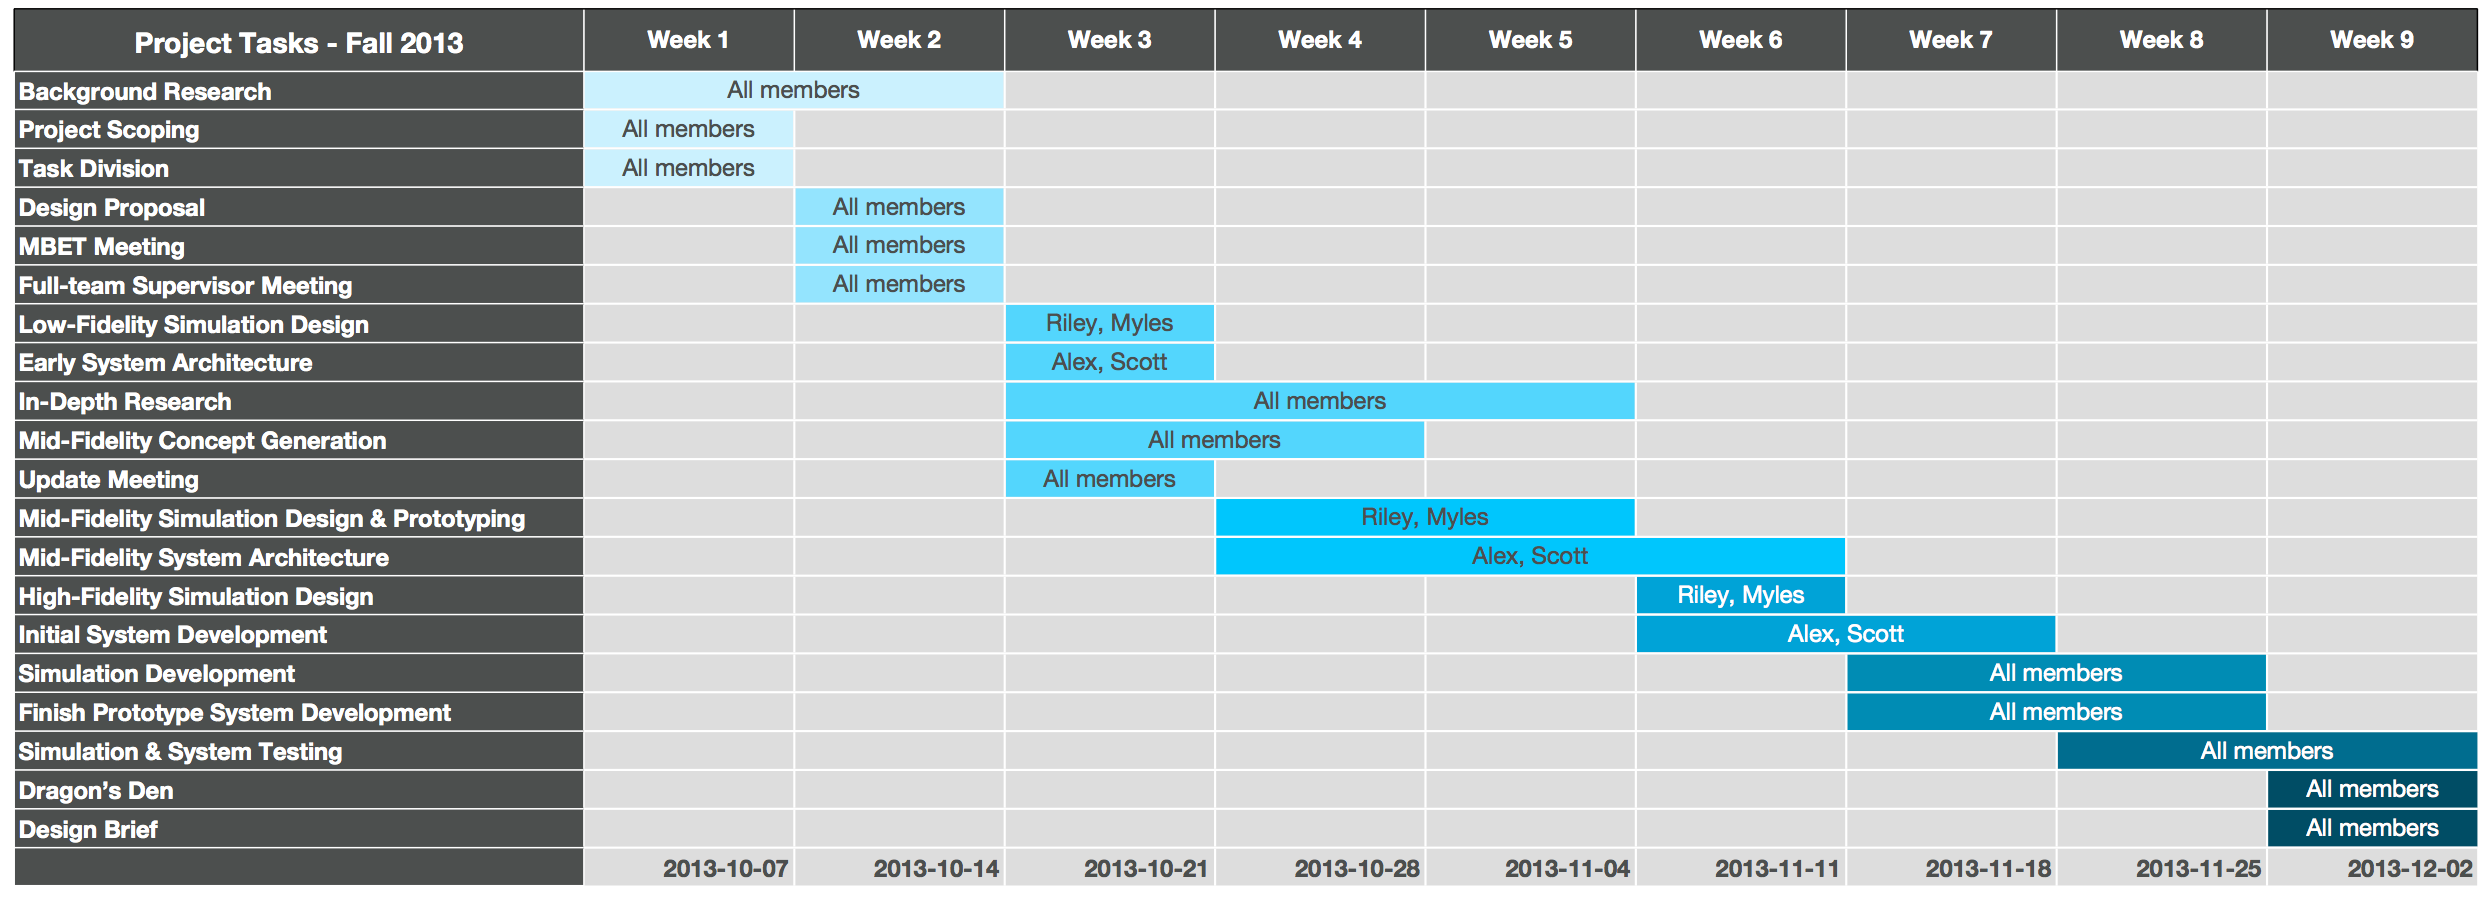
\includegraphics[scale=0.22, angle = 90]{figures/gantt-fall.png}
\caption{Gantt Chart for Fall 2013.}
\label{fig:gantt-fall}
\end{figure}

\newpage
\subsection{Gantt Chart}
\begin{figure}[H]
  \begin{centering}
    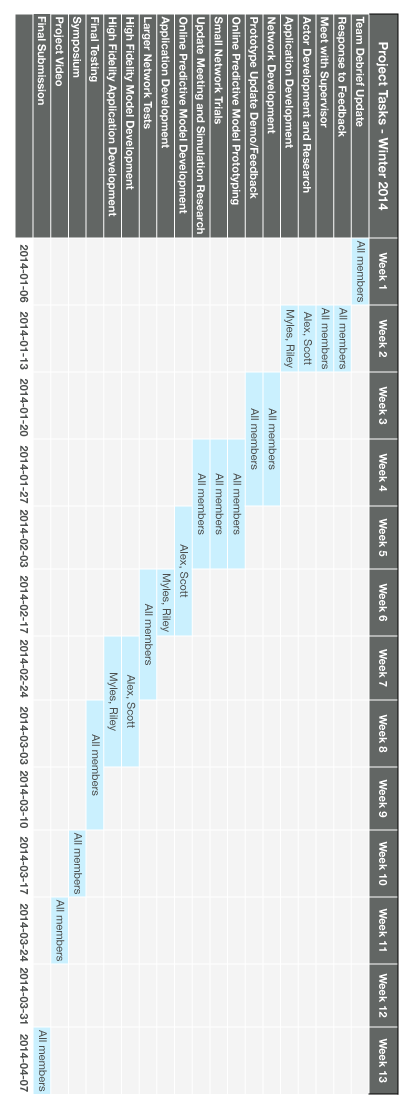
\includegraphics[scale=0.5, angle=180]{figures/gantt-vertical.png}
    \caption{Gantt Chart for Winter 2014}
    \label{fig:gantt-winter}
  \end{centering}
\end{figure}

\subsection{Performance Review}

\newpage
\section{Conclusion}

\newpage
\addcontentsline{toc}{section}{References}

\bibliographystyle{IEEEtran}

\bibliography{bib}

\end{document}
